%===============================================================================
% Authors: 2008 Michal Bidlo, 2019 Jaroslav Dytrych, 2021 Dominik Harmim
% Contact for questions and comments: sablona@fit.vutbr.cz
% Author contact: xharmi00@stud.fit.vutbr.cz
%===============================================================================
% encoding: UTF-8
%-------------------------------------------------------------------------------
% processing: make, make all, make pdf, make xharmi00.pdf make clean, make pack
%             make xharmi00.tar.gz, make vlna, make normostrany
%===============================================================================
% Included files:
%   xharmi00.bib - bibliography
%   xharmi00-chapters.tex - the thesis content
%   xharmi00-appendices.tex - appendices
%===============================================================================


\documentclass[british, zadani, odsaz]{fitthesis}


% Basic packages are at the bottom of template file fitthesis.cls.
\usepackage{wrapfig}
\usepackage{amsthm}
\usepackage[ruled, algochapter, linesnumbered]{algorithm2e}
% \usepackage{tocloft}

% Setting of a path to the pictures.
\graphicspath{{img/}}

\renewcommand{\rmdefault}{lmr} % set Latin Modern Roman as rm
\renewcommand{\sfdefault}{qhv} % set TeX Gyre Heros as sf
\renewcommand{\ttdefault}{lmtt} % set Latin Modern tt as tt

% Definition theorem.
\theoremstyle{definition}
\newtheorem{definition}{Definition}[section]

% Example theorem.
\theoremstyle{definition}
\newtheorem{example}{Example}[section]

% Algorithm margin.
\setlength{\algomargin}{2em}

% Line spacing in the table of contents.
% \renewcommand\cftchapafterpnum{\vskip .5em}
% \renewcommand\cftsecafterpnum{\vskip .5em}

% "hyperref" package create clickable links in pdf if you are using pdflatex.
% Problem is that this package have to be introduced as the last one so it
% cannot be placed in the template file.
\ifWis
    \ifx\pdfoutput\undefined\else
        \usepackage[
            unicode, colorlinks, hyperindex, plainpages=false, pdftex
        ]{hyperref}
        \definecolor{hrcolor-ref}{RGB}{223, 52, 30}
        \definecolor{hrcolor-cite}{HTML}{2F8F00}
        \definecolor{hrcolor-urls}{HTML}{092EAB}
        \hypersetup{
            linkcolor=hrcolor-ref, citecolor=hrcolor-cite, filecolor=magenta,
            urlcolor=hrcolor-urls
        }
    \fi
\else % for the print clickable links will be black
    \ifx\pdfoutput\undefined\else
        \usepackage[
            unicode, colorlinks, hyperindex, plainpages=false, pdftex,
            urlcolor=black, linkcolor=black, citecolor=black
        ]{hyperref}
        \definecolor{links}{rgb}{0, 0, 0}
        \definecolor{anchors}{rgb}{0, 0, 0}
        \def\AnchorColor{anchors}
        \def\LinkColor{links}
    \fi
\fi

% This solves the problems with links which leads after the picture.
\usepackage[all]{hypcap}

% Solves first/last row of the paragraph on the previous/next page.
\clubpenalty=10000
\widowpenalty=10000


% Information about the thesis
%-------------------------------------------------------------------------------
\projectinfo{%
    % Thesis
    project={SP}, % thesis type
    year={2021}, % year of a submission
    date=\today, % submission date
    faculty={FIT}, % name of the faculty
    department={UITS}, % appropriate abbreviation of the department
%
    % Thesis title
    % thesis title in english
    title.en={%
        Advanced Static Analysis of Atomicity in Concurrent Programs through
        Facebook Infer%
    },
    % thesis title in czech language
    title.cs={%
        Pokročilá statická analýza atomičnosti v~paralelních programech
        v~prostředí Facebook Infer%
    },
    % setting the length of a block with a thesis title
    title.length={15cm},
    % setting the length of a block with a second thesis title
    sectitle.length={15cm},
%
    % Author
    author.name={Dominik}, % author name
    author.surname={Harmim}, % author surname
    author.title.p={Bc.}, % title before the name
%
    % Supervisor
    supervisor.name={Tomáš}, % supervisor name
    supervisor.surname={Vojnar}, % supervisor surname
    supervisor.title.p={prof. Ing.}, % title before the name
    supervisor.title.a={Ph.D.}, % title after the name (optional)
%
    % Keywords
    % keywords in english
    keywords.en={%
        Here, individual keywords separated by commas will be written in
        English.%
    },
    % keywords in czech language
    keywords.cs={%
        Sem budou zapsána jednotlivá klíčová slova v~českém (slovenském)
        jazyce, oddělená čárkami.%
    },
%
    %Abstract
    abstract.en={%
        An abstract of the work in English will be written in this paragraph.%
    },
    abstract.cs={%
        Do tohoto odstavce bude zapsán výtah (abstrakt) práce v~českém
        (slovenském) jazyce.%
    },
%
    % Extended abstract
    extendedabstract={%
        Do tohoto odstavce bude zapsán rozšířený výtah (abstrakt) práce
        v~českém (slovenském) jazyce.%
    },
%
    % Declaration
    declaration={%
        I~hereby declare that this Bachelor's thesis was prepared as an
        original work by the author under the supervision of Mr. X.
        The supplementary information was provided by Mr. Y.
        I~have listed all the literary sources, publications and other sources,
        which were used during the preparation of this thesis.%
    },
%
    % Acknowledgement
    acknowledgement={%
        Here it is possible to express thanks to the supervisor and to the
        people which provided professional help (external submitter,
        consultant, etc.).%
    }
}


% Additional hyperref settings.
\ifx\pdfoutput\undefined\else
    \def\pdfBorderAttrs{/Border [0 0 0]} % without margins around links
    \pdfcompresslevel=9
    \hypersetup{
        pdfauthor=\pdfauthor,
        pdftitle=\pdftitle,
        pdfsubject=\pdfsubject,
        pdfkeywords=\pdfkeywords
    }
\fi


%===============================================================================
\begin{document}
    % Typesetting of the title pages
    % --------------------------------------------------------------------------
    \maketitle


    % Table of contents
    % --------------------------------------------------------------------------
    \setlength{\parskip}{0pt}
    \pagenumbering{roman}

    {\hypersetup{hidelinks}\tableofcontents}

    \ifODSAZ
        \setlength{\parskip}{.5\bigskipamount}
    \else
        \setlength{\parskip}{0pt}
    \fi


    \iftwoside\cleardoublepage\else\clearpage\fi


    % Thesis text
    % --------------------------------------------------------------------------
    \pagenumbering{arabic}
    \setcounter{page}{1}

    %===============================================================================
% (c) Dominik Harmim


%===============================================================================



\chapter{Introduction}

Bugs have been present in computer programs ever since the inception of the programming discipline. Unfortunately, they are often hidden in unexpected places, and they can lead to unexpected behaviour, which may cause significant damage. Nowadays, developers have many possibilities of catching bugs in the early development process. \emph{Dynamic analysers} or tools for \emph{automated testing} are often used, and they are satisfactory in many cases. Nevertheless, they can still leave too many bugs undetected because they can analyse only \emph{particular program flows} dependent on the input data. An alternative solution is \emph{static analysis} (despite it, of course, suffers from some problems too\,---\,such as the possibility of reporting many \emph{false alarms}, i.e., \emph{spurious errors}). Quite some tools for static analysis were implemented, e.g., Coverity or CodeSonar. However, they are often proprietary and difficult to openly evaluate and extend.

Recently, Facebook introduced \emph{Facebook Infer}: an \emph{open-source} tool for creating \emph{highly scalable}, \emph{compositional}, \emph{incremental}, and \emph{interprocedural} static analysers. Facebook Infer has grown considerably, but it is still under active development by many teams across the globe. It is employed every day not only in Facebook itself but also in other companies, such as Spotify, Uber, Mozilla, or Amazon. Currently, Facebook Infer provides several analysers that check for various types of bugs, such as buffer overflows, data races and some forms of deadlocks and starvation, null-dereferencing, or memory leaks. However, most importantly, Facebook Infer is a~\emph{framework} for building new analysers quickly and easily. Unfortunately, the current version of Facebook Infer still lacks better support for \emph{concurrency bugs}. While it provides a~reasonably advanced data race analyser, it is limited to Java and C++ programs only and fails for C~programs, which use a~\emph{lower-level lock manipulation}. Moreover, the only available checker of \emph{atomicity of call sequences} is the first version of \emph{Atomer}~\cite{harmimBP} proposed in the bachelor's thesis of the author.

At the same time, in \emph{concurrent programs}, there are often \emph{atomicity requirements} for the execution of specific sequences of instructions. Violating these requirements may cause many kinds of problems, such as unexpected behaviour, exceptions, segmentation faults, or other failures. \emph{Atomicity violations} are usually not verified by compilers, unlike syntactic or some sorts of semantic rules. Moreover, atomicity requirements, in most cases, are not even documented at all. Therefore, in the end, programmers themselves must abide by these requirements and usually lack any tool support. Furthermore, in general, it is difficult to avoid errors in \emph{atomicity-dependent programs}, especially in large projects, and even more laborious and time-consuming is finding and fixing them. The papers~\cite{contracts2017, atomizer, contracts2015, atomicityOOP} discuss the importance of \emph{atomicity-related bugs}, and they also show some bugs in \emph{real-world programs}. Unfortunately, tool support for automatically discovering such kinds of errors is currently minimal.

As already mentioned, within the author's bachelor's thesis~\cite{harmimBP}, \emph{Atomer}\footnote{The implementation of~\textbf{Atomer} is available at GitHub as an \emph{open-source} repository (in a~branch \texttt{atomicity-sets}): \url{https://github.com/harmim/infer}.} was proposed\,---\,a~\emph{static analyser} for finding some forms of \emph{atomicity violations} implemented as a~Facebook Infer's module. In particular, the stress is put on the \emph{atomic execution of sequences of function calls}, which is often required, e.g., when using specific library calls. For example, assume the function \texttt{replace} from Listing~\ref{list:exampleViolation} that replaces item~\texttt{a} in an array by item~\texttt{b}. It contains atomicity violation\,---\,the index obtained may be outdated when \texttt{set} is executed (because, e.g., a~\emph{concurrent thread} can modify the array), i.e., \texttt{index\_of} and \texttt{set} should be executed atomically. The analysis is based on the assumption that sequences of function calls executed \emph{atomically once} should probably be executed \emph{always atomically}. Hence, the checker naturally works with sequences. In fact, the idea of checking the atomicity of certain sequences of function calls is inspired by the works of \emph{contracts for concurrency}~\cite{contracts2017, contracts2015}. In the terminology of~\cite{contracts2017, contracts2015}, the atomicity of specific sequences of calls is the most straightforward (yet very useful in practice) kind of contracts for concurrency. However, while the idea of using sequences in the given context is indeed natural and rather exact, it quite severely limits the \emph{scalability} of the analysis (indeed, even with a~few functions, there can appear numerous different orders in which they can be called). Moreover, the implementation of the first version of Atomer targets mainly \emph{C~programs} using \emph{PThread locks}. Consequently, there was no support for other languages and their locking mechanisms in the first version of Atomer.

\begin{lstlisting}[style=c++, label={list:exampleViolation}, float=hbt, caption={An example of \emph{atomicity violation}}]
void replace(int a, int b, Array &array) 
{
    int i = array.index_of(a);
    if (i >= 0) array.set(i, b);
}
\end{lstlisting}

Within this thesis, Atomer has been \emph{significantly improved and extended}. In particular, to improve scalability, working with \emph{sequences} of function calls was \emph{approximated} by working with \emph{sets} of function calls. Furthermore, several new features were implemented: support for \emph{C++ and Java}, including various advanced kinds of \emph{locks} these languages offer (such as \emph{re-entrant locks} or \emph{lock guards}); or a~more precise way of \emph{distinguishing between different lock instances}. Moreover, the analysis has been \emph{parameterised} by function names to concentrate on during the analysis and limits of the number of functions in \emph{critical sections}. These parameters aim to reduce the number of false alarms. Their proposal is based on the author's analysis of false alarms produced by the first Atomer's version. Lastly, new experiments were performed to test capabilities of the new version of Atomer.

The development of the original Atomer started under the H2020 ECSEL projects AQUAS and Arrowhead Tools. The development of its new version is supported by the H2020 ECSEL project VALU3S. It has been discussed with the developers of Facebook Infer too. Parts of the thesis concerning the preliminaries and the basic version of Atomer are partially taken from the thesis~\cite{harmimBP}. Moreover, some preliminary results were also published in the Excel@FIT paper~\cite{excel2021Harmim} written by the author.

The rest of the thesis is organised as follows. Chapter~\ref{chap:prelim} describes all the topics related to and essential to this thesis (including \emph{static analysis}, \emph{abstract interpretation}, \emph{Facebook Infer}, and \emph{contracts for concurrency}). The original version of \emph{Atomer}, its limitations, and related work are described in Chapter~\ref{chap:atomer}. Subsequently, Chapter~\ref{chap:proposal} presents all the proposed extensions and improvements. The implementation of these extensions is then covered in Chapter~\ref{chap:implement}. The experimental evaluation of the new Atomer's features and other experiments performed within this thesis are discussed in Chapter~\ref{chap:exp} together with the future work. Finally, the thesis is concluded in Chapter~\ref{chap:conc}. Besides, there are included the following appendices. The content of the attached memory media is listed in Appendix~\ref{app:memMedia}. In the end, Appendix~\ref{app:man} serves as an installation and user manual.



%===============================================================================


\chapter{Preliminaries}
\label{chap:prelim}

This chapter explains the theoretical background that the thesis builds on. It also explains and describes the existing tools used in the thesis. Also, note that the author already partially published the contents of the sections in this chapter in his bachelor's thesis~\cite{harmimBP} and paper~\cite{excel2021Harmim}.

\paragraph{Multi-Threaded Programs~\cite{atomizer, muzikovskaBP}}
\emph{Multiple threads} of control are commonly used in the software development process because they help reduce \emph{latency}, increase \emph{throughput}, and better utilise \emph{multiple processor computers}. Threads or \emph{processes} are independent \emph{sequences of instructions} that may be performed simultaneously. A~process represents a~single running program. It has its own address space and a~unique identifier. One process can consist of multiple threads, i.e., a~thread is a~so-called \emph{lightweight process}. All threads of a~single process share the same address space (i.e., code and data). However, reasoning about the behaviour and correctness of a~multi-threaded system is complex due to the need to consider all possible interleavings of the executions of different threads. An integral part of parallel programming is the \emph{synchronisation} of individual threads. Usually, synchronisation mechanisms ensure the \emph{mutual exclusion} of shared resources or synchronise actions that threads perform. Operating systems provide basic synchronisation primitives that can be often used in programming languages in a~higher-level manner. Such fundamental mechanisms are \emph{semaphores} (binary semaphores are called \emph{mutexes}), \emph{barriers}, \emph{read-copy-update} techniques, or \emph{monitors}. In this work (and also in practice), for simplicity, it will be used a~notion of \emph{locks} for semaphores, mutexes, monitors, etc. as a~mechanism that mutually excludes access to a~\emph{critical section}.

The use of locks and access to shared data in parallel programs involves the risk of errors not known in sequential programming. Much previous work on checking \emph{thread interference} has focused on \emph{data races} (or, in general, on \emph{race conditions}). A~data race occurs when two threads simultaneously access the same data variable, and, at least, one of the access is a~write. In practice, data races are commonly avoided by guarding each data structure with a~lock. Unfortunately, the absence of data races is insufficient to guarantee the absence of errors due to unexpected interference between threads.~\cite{atomizer, atomicityOOP}

\paragraph{Atomicity Violations~\cite{atomizer}}
Another possible source of errors due to unexpected interference between threads are \emph{atomicity violations}. A~method (or, in general, a~code block) is \emph{atomic} iff, for every (arbitrarily interleaved) program execution, there is an equivalent execution with the same overall behaviour where the atomic method is executed serially. In other words, the method's execution is not interleaved with instructions of other threads. Also, atomicity provides a~powerful, indeed maximal, guarantee of non-interference among threads. In short, atomicity is a~generally applicable and fundamental \emph{correctness property} of multi-threaded code. Nevertheless, commonly used \emph{testing approaches} are deficient in verifying atomicity. While testing may reveal a~concrete interleaving in which an atomicity violation causes erroneous behaviour, the exponentially large amount of possible interleavings does fundamentally impossible to get suitable \emph{test coverage}. Research results~\cite{contracts2017, atomizer, contracts2015, atomicityOOP} have shown that defects related to atomicity are common, even in well-tested libraries.

It has to be described which blocks of code should be executed atomically to detect atomicity violations. Algorithms for the detection of this error often deal only with the atomicity of operations on variables. Examples of a~complex description of \emph{atomicity requirements} are \emph{contracts} that require atomicity of the execution of certain methods/functions (defined in Section~\ref{sec:contracts}).~\cite{muzikovskaBP}

Further, Section~\ref{sec:programAnalysis} outlines the fundamental notions and approaches in \emph{program analysis}. In Section~\ref{sec:AI}, there is an explanation of \emph{static analysis} by \emph{abstract interpretation}, which is used in \emph{Facebook Infer}, i.e., the key framework used in this thesis. Facebook Infer, its principles, and features are covered in Section~\ref{sec:fbinfer}. The concept of \emph{contracts for concurrency} is discussed and defined in Section~\ref{sec:contracts}.


\section{Concepts in Program Analysis}
\label{sec:programAnalysis}

This section provides a~fundamental intuition about the main principles of \emph{program analysis}. It discusses several standard techniques for reasoning about programs. The section is based on a~few first chapters from the book~\cite{staticAnalysisRival} and the overview paper~\cite{analysisAndVerVojnarKrena}.

\subsection{What to Analyse}

The first question is \emph{what programs to analyse}. An obvious characterisation of programs to analyse is the programming language in which the programs are written. Moreover, certain specific families of input programs may be distinguished. However, besides the language and the family of programs to consider, the way input programs are processed can also differ and affects how the analysis works. The most straightforward way to handle input programs is working directly with a~\emph{source code} just like a~compiler would. Nevertheless, different representations of programs are used in program analysis likewise. The two below types of techniques are customarily distinguished.

\paragraph{Program-Level Analysis}
The first possibility is to run the analysis on a~\emph{source code} of input programs (e.g., programs written in conventional programming languages like~C or Java; or hardware described in VHDL, Verilog, etc.) or on \emph{executable binaries}. This technique typically involves some \emph{front-end} comparable to a~compiler's one that constructs the \emph{syntax trees} of input programs.

\paragraph{Model-Level Analysis}
An alternative option is to consider a~different input language that aims at modelling the semantics of programs. Then, the analysis takes as an input a~description that \emph{models} the program to analyse. Such models either need to be created manually, or some specialised tools are used. These models may hide implementation difficulties or inaccuracies. Examples of the models are automata of any kind, UML diagrams, Petri nets, Markov chains, or specialised modelling languages like, e.g., Promela.

\subsection{Static vs Dynamic Approaches}

Another critical question in program analysis is \emph{when} the analysis is made. In particular, whether it operates \emph{during} or \emph{before} the program's execution.

One solution is to analyse programs at \emph{run-time}, i.e., \emph{during} the program's execution. This approach is called \emph{dynamic analysis}. It takes place while the program computes, often, over a~number of executions.

A~second approach is to analyse the program \emph{before} execution, which is called \emph{static analysis}. It is done independently from any execution.

Static and dynamic approaches are significantly distinct in many ways. They come with different benefits and weaknesses. While dynamic approaches are often simpler to design and implement, they often have problems with performance at run-time. They do not force developers to fix bugs before program execution. Moreover, some properties cannot be checked (or, at least, it is very challenging) dynamically. For instance, dynamically detecting whether an execution does not \emph{terminate} would require an infinite program run. Particular static and dynamic techniques are further discussed in Section~\ref{sec:analysisTechniques}.

\subsection{Automation and Scalability}

\emph{Automation} is a~further relevant aspect in program analysis. It would be ideal if program analysis methods were \emph{fully automated} (i.e., no human help is needed). Unfortunately, this is not always possible due to the consequences of \emph{Rice's theorem}~\cite{rice}. Thus, sometimes, it is needed to give up on automation and let program analyses ask some \emph{user input} (i.e., some human help is required). In that case, the user is asked to give some information to the analysis, e.g., \emph{invariants}\footnote{An \textbf{invariant} is a~\emph{logical property} that can be proved to be inductive for a~given program.}. That is, the analysis is partially manual since users need to compute parts of the results themselves. However, having to provide this information may be unwieldy because input programs can be huge or complex.

\emph{Scalability} is another essential characteristic of program analysis algorithms. Even if a~program analysis is fully automatic, it is not guaranteed that it will generate a~result within a~reasonable time, depending on the complexity of the algorithms. A~program analysis tool may not \emph{scale} to extensive programs due to time costs or, e.g., memory constraints.

\subsection{Soundness and Completeness}

In order to preserve automation and/or scalability, the conditions about program analysis may be relaxed. Namely, the analysis can be proposed to return \emph{inaccurate} results (alternatively, it can return a~non-conclusive \uv{do not know} answer). For this purpose, two dual properties (forms of \emph{approximations} or \emph{inaccuracies}) are used. To express these notions, let~$ \mathcal{L} $ be a~\emph{Turing-complete language}, $ \varphi $ be a~\emph{non-trivial semantic property} of interest of programs of~$ \mathcal{L} $, and~$ T $ be an analysis tool that decides whether~$ \varphi $ holds in a~given program. Ideally, if~$ T $ were absolutely precise, it would be such that:
$$
    \text{for every program}\ P \in \mathcal{L}: T(P) = true \Longleftrightarrow P \models \varphi
$$
The above, of course, can be decomposed into a~pair of implications:
$$
    \begin{cases}
        \forall P \in \mathcal{L}: T(P) = true \Longrightarrow P \models \varphi \\
        \forall P \in \mathcal{L}: T(P) = true \Longleftarrow P \models \varphi
    \end{cases}
$$

\paragraph{Soundness}
A~\emph{sound} program analysis satisfies the first implication.
\begin{definition}[\textbf{Soundness}~\cite{staticAnalysisRival}]
    The program analyser~$ T $ is sound w.r.t. property~$ \varphi $ whenever, for any program $ P \in \mathcal{L} $, $ T(P) = true \Longrightarrow P \models \varphi $.
\end{definition}
When a~sound analysis terminates and claims that the analysed program has property~$ \varphi $, it guarantees that the program indeed satisfies~$ \varphi $, i.e., no errors are missed. In other words, a~sound analysis will refuse all programs that do not satisfy~$ \varphi $. In terms of errors in \emph{binary classification}, there are not \emph{false-negative} errors\footnote{A~\textbf{false-negative} error is a~real error that is undetected by an analysis tool.} when using sound analysis. On the other hand, there is a~chance of \emph{false-positive} errors\footnote{A \textbf{false-positive} error (also called a~\textbf{false alarm}) is a~\emph{spurious error}, i.e., it is detected by an analysis tool, but the error does not exist in the real program.}.

\paragraph{Completeness}
A~\emph{complete} program analysis satisfies the second implication.
\begin{definition}[\textbf{Completeness}~\cite{staticAnalysisRival}]
    The program analyser~$ T $ is complete w.r.t. property~$ \varphi $ whenever, for any program $ P \in \mathcal{L} $, $ P \models \varphi \Longrightarrow T(P) = true $.
\end{definition}
A~complete program analysis will accept every program that satisfies property~$ \varphi $. In other words, when a~complete analysis refuses an analysed program, it is guaranteed that the program indeed fails to satisfy~$ \varphi $, i.e., there are no false-positive errors. However, there can be false-negative errors.

Due to the \emph{computability} barrier~\cite{rice}, it is not possible to design a general analysis to determine which programs satisfy any non-trivial property for a~Turing-complete language that is sound, complete, fully automated, and scalable at the same time. Some of these have to be sacrificed, or the analysis has to be proposed to operate only on a~specific set of input programs.

\subsection{Program Analysis Techniques}
\label{sec:analysisTechniques}

This section describes several standard \emph{program analysis techniques}. Although this thesis focuses on \emph{static analysis} (or maybe rather \emph{bug finding} based on static analysis), it is essential to see the differences between other analysis techniques. Hence, a~brief overview is presented in the below sections. Finally, Table~\ref{tab:progAnalysisTechniques} compares the techniques (how they are usually used) based on the earlier criteria.

\paragraph{Testing and Dynamic Analysis}
The \emph{testing} approach checks a~finite set of finite program executions. In the development process, several levels of testing are used at various stages of the software/hardware life-cycle, e.g., \emph{unit testing} or \emph{integration testing}. In general, it is challenging to achieve suitable \emph{test coverage} because of infinite program paths when using, e.g., \emph{random testing}. However, several more advanced techniques that improve the coverage have been introduced. These techniques are often combined with other verification approaches. For instance, \emph{concolic testing} combines testing with \emph{symbolic execution}, \emph{dynamic analysis} that observes behaviour in a~testing run (such behaviour can be \emph{extrapolated} to behaviour not seen in the given testing run), or \emph{search-based techniques} that can generate test data or parameters. Moreover, to test programs with non-deterministic semantics (i.e., concurrent programs), techniques like \emph{noise injection} are applied. In particular, many advanced dynamic analysers have been proposed to detect data races or deadlocks, including, e.g., Eraser or FastTrack.

Testing has the following features. In general, it is simple to automate. It is unsound in almost all cases (besides programs that have a~finite number of finite paths). Since failed testing runs provide incorrect concrete executions, the testing is complete.

Other analysis techniques mentioned below use a~static approach. The significant difference between static and dynamic approaches is the following. It is well-known that testing may expose errors, but it cannot prove their absence. It was also famously stated by Edsger W. Dijkstra: \uv{\textit{Program testing can be used to show the presence of bugs, but never to show their absence!}}. However, static approaches may be able to prove their absence\,---\,with some \emph{approximation}\,---\,they can check \emph{all possible executions} of a~program and provide guarantees about its properties. Another static approaches' benefit is that the analysis can be performed during the development process, so the program does not have to be executable yet, and it already can be analysed. The biggest drawback of static approaches, in general, is that they can produce a~lot of false alarms (though this is not the case, e.g., for \emph{theorem proving}), which is often resolved by accepting unsoundness. Another crucial issue of static approaches (this is, however, also an issue of dynamic analyses) is ensuring sufficient scalability\,---\,in fact, typically, the more precise the analysis, the less scalable it becomes.

\paragraph{Deductive Verification}
The \emph{semi-automated} approach \emph{deductive verification} (or \emph{theorem proving}) uses \emph{inference systems} for inferring theorems about the analysed system from the facts known about the system and from general theorems of different logical theories. The approach falls under \emph{machine-assisted} techniques, which means that users may be required to provide extra information to the analysis (usually \emph{loop invariants}, procedure \emph{preconditions/postconditions}, assertions, or some other invariants). This can be demanding and require some level of expertise. However, a~substantial part of the verification can usually still be carried out in a~fully automated fashion. This approach is very general, but there is a~problem with generating diagnostic information for incorrect systems. There exist a~number of \emph{interactive theorem proving} tools like Coq, Isabelle/HOL, PVS, ACL2, etc. The user usually guides the inference process in these tools.

These techniques also involve \emph{automated decision procedures} (or \emph{satisfiability solvers}) for various logical theories. Such solvers are often used as back-end components for higher-level verification methods, such as \emph{symbolic execution} or \emph{predication abstraction} in model checking. Commonly used solvers are \emph{SAT-solvers} (e.g., CaDiCaL and Glucose) and \emph{SMT-solvers} (e.g., Z3 and CVC4). Various tools allow the user to provide some \emph{logical annotations} in a~code and then automatically attempt to prove specific properties using decision procedures. Examples of such tools are VCC and Dafny.

Theorem proving techniques have the following properties. They are not fully automatic, i.e., \emph{high user expertise} is often needed. They are sound w.r.t. the model of the program used in the proof, and they are usually complete up to the capabilities of the proof assistant.

\paragraph{Model Checking}
Another technique called (\emph{finite-state}) \emph{model checking} aims at finite systems. It automatically verifies  whether a~system or its model satisfies a~particular property based on an \emph{algorithmic exploration of the system's state space}. Unfortunately, the biggest issue here is the \emph{state space explosion} problem~\cite{stateExpl}. However, in practice, model checking tools use effective data structures (such as \emph{binary decision diagrams} or \emph{hierarchical storage of states}) to describe program behaviours and avoid enumerating all executions thanks to approaches that reduce the search space. In addition, other techniques are used to cope with this problem. For instance, various abstractions are used (e.g., \emph{predicate abstraction}) or \emph{bounded model checking}\footnote{\textbf{Bounded model checking} explores models up to a~\emph{fixed depth} only. This technique is often referred to as \emph{bug finding} because it sacrifices completeness and often also soundness. Examples of tools that implement such technique are CMBC, LLBMC, or JBMC.}. Properties are usually defined using \emph{temporal logics}, such as LTL, CTL, or PCTL. Finite model checking has the following characteristics. It is automatic (up to the need of modelling the system or its environment). It is sound and usually complete, w.r.t. the model. Other advantages are that it is pretty general and provides diagnostic data for incorrect systems.

Model checking is typically done at the \emph{model level}, i.e., a~model of the program needs to be built, either manually or automatically. In practice, model checking tools usually implement a~front-end for that purpose. The problem is that the model generally cannot precisely capture the input program's behaviours since programs are usually infinite systems. Thus, the checking of the synthesised model may be either incomplete or unsound, w.r.t. the input program. Some model checking techniques can automatically \emph{refine} the model when they fail to prove a~property due to a~\emph{spurious counterexample}, although a~\emph{termination} must be ensured. In practice, model checking tools are often sound and incomplete w.r.t. the input program.

Model checking has found many successful applications, including hardware verification, verification of \emph{concurrent} and \emph{distributed} systems, \emph{probabilistic} systems, \emph{biological} systems, etc. Examples of hardware model checkers are RuleBase, Incisive Verifier, or NuSMV. Model checkers for concurrent and distributed systems include Spin or DIVINE. Tools, such as CPAchecker or BLAST, are model checkers that use predicate abstraction. PRISM and Storm are state-of-the-art tools for model checking probabilistic systems. Finally, Uppaal is a~model checker that verifies temporal logic formulas on \emph{timed automata}.

\paragraph{Static Analysis}
...

\begin{table}[hbt]
    \centering

    \begin{tabular}{|l|c|c|c|c|c|}
        \hline
        \textbf{Technique} & \textbf{Automatic} & \textbf{Sound} & \textbf{Complete} & \textbf{Object} & \textbf{Approach} \\ \hline \hline
        Testing & Yes & No & Yes & Program & Dynamic \\ \hline
        Deductive & \multirow{2}{*}{No} & \multirow{2}{*}{Yes} & \multirow{2}{*}{Yes/No} & \multirow{2}{*}{Model/Program} & \multirow{2}{*}{Static} \\
        verification & & & & & \\ \hline
        Model checking & Yes & Yes & Yes/No & Model/Program & Static \\ \hline
        Conservative & \multirow{2}{*}{Yes} & \multirow{2}{*}{Yes} & \multirow{2}{*}{No} & \multirow{2}{*}{Program} & \multirow{2}{*}{Static} \\
        static analysis & & & & & \\ \hline
        Bug finding & Yes & No & No & Program & Static \\ \hline
    \end{tabular}

    \caption{A~summary of \emph{program analysis techniques}~\cite{staticAnalysisRival}}
    \label{tab:progAnalysisTechniques}
\end{table}


\section{Abstract Interpretation}
\label{sec:AI}

\todo{Přidat Galoisovo spojení. Definovat widening, narrowing.}

According to~\cite{staticAnalysisMoller}, \emph{static analysis} of
programs is reasoning about the behaviour of computer programs without
actually executing them. It has been used since the 1970s in optimising
compilers for generating efficient code. More recently, it has proven
valuable also for automatic error detection, verification of correctness
of programs, and it is used in other tools that can help programmers.
Intuitively, a~static program analyser is a~program that reasons about the
behaviour of other programs, in other words, a~static program analyser is
a~program that reasons about another programs by looking for some
\emph{syntactic patterns} in the code and/or by assigning the program
statements some \emph{abstract semantics} and then deriving
a~characterisation of the behaviour in terms of the abstract semantics.
Nowadays, static analysis is one of the fundamental concepts of
\emph{formal verification}. It aims to automatically answer questions
about a~given program, such as, e.g.,~\cite{staticAnalysisMoller}:
\begin{itemize}
    \item
        \textbf{Are certain operations executed \emph{atomically}?}

    \item
        Does the program terminate on every input?

    \item
        Can the program \emph{deadlock}?

    \item
        Does there exist an input that leads to a~\emph{null-pointer
        dereference}, a~\emph{division-by-zero}, or an \emph{arithmetic
        overflow}?

    \item
        Are all variables initialised before they are used?

    \item
        Are arrays always accessed within their bound?

    \item
        Does the program contain \emph{dead code}?

    \item
        Are all resources correctly released after their last
        use?
\end{itemize}

Various forms of static analysis of programs have been invented, for
instance~\cite{harmimBP}: bug pattern searching, data-flow
analysis, constraint-based analysis, type analysis, or symbolic execution.
One of the most widely used approaches\,---\,\emph{abstract
interpretation}\,---\,is detailed in Section~\ref{sec:AI}.

There exist numerous tools for static analysis (often proprietary and
difficult to openly evaluate or extend), e.g.: Coverity, Klockwork, CodeSonar,
Frama-C, PHPStan, or \emph{Facebook Infer} (described in
Section~\ref{sec:fbinfer}).

\subsection{Abstract Interpretation}

\todo{Pro definici summary citovat Hoareho a~použít jeho trojice.}

This section explains and defines the basics of \emph{abstract interpretation}.
The description is based on~\cite{AIBasedFormalMethodsCousot,
AILatticeModelCousot, AIInNutshellCousot, AICousotWeb, savAI,
harmimBP, wideningNarrowingCousot, programAnalysisNielson,
staticAnalysisMoller}. In these works, there can be
found more detailed and more formal explanation.

Abstract interpretation was introduced and formalised by a~French
computer scientist Patrick Cousot and his wife Radhia Cousot in the year
1977 at POPL (symposium on Principles of Programming
Languages)~\cite{AILatticeModelCousot}. It is a~generic \emph{framework}
for static analyses. It allows one to create particular analyses by
providing specific components (described later) to the framework. The
obtained analysis is guaranteed to be \emph{sound} if certain properties
of the components are met.~\cite{savAI, harmimBP}

In general, in the set theory, which is independent of the application
setting, abstract interpretation is considered a~theory for
\emph{approximating} sets and set operations. A~more restricted formulation
of abstract interpretation is to interpret it as a~theory of approximation
of the behaviour of the \emph{formal semantics} of programs. Those
behaviours may be characterised by \emph{fixpoints} (defined below), which
is why a~primary part of the theory provides efficient techniques for
\emph{fixpoint approximation}~\cite{programAnalysisNielson}.
So, for a~standard semantics, abstract interpretation is used to derive
the approximate abstract semantics over an \emph{abstract domain} (defined
below). The abstract semantics obtained as a~result of program analysis can
then be used for verification, optimisation, code generation or
transformation, etc.~\cite{AIBasedFormalMethodsCousot}

Patrick Cousot intuitively and informally illustrates abstract
interpretation in~\cite{AIInNutshellCousot} as follows.
Figure~\ref{fig:ai1} shows the \emph{concrete semantics} of a~program
by a~set of curves, which represents the set of all possible executions
of the program in all possible execution environments. Each curve shows
the evolution of the vector~$ x(t) $~of input values, state, and
output values of the program as a~function of the time~$ t $.
\emph{Forbidden zones} on this figure represent a~set of erroneous states
of the program execution. Proving that the intersection of the concrete
semantics of the program with the forbidden zone is empty may be
\emph{undecidable} because the program concrete semantics is, in general,
\emph{not computable}. As demonstrates Figure~\ref{fig:ai2}, abstract
interpretation deals with an \emph{abstract semantics}, i.e., the
\emph{superset} of the concrete program semantics. The abstract semantics
includes all possible executions. That implies that if the abstract
semantics is safe (i.e. it does not intersect the forbidden zone), the
concrete semantics is safe as well. However, the \emph{over-approximation}
of the possible program executions causes that inexisting program executions
are considered, which may lead to \emph{false alarms}. It is the case when
the abstract semantics intersects the forbidden zone, whereas the concrete
semantics does not intersect it.

\begin{figure}[hbt]
    \centering

    \begin{subfigure}[hbt]{.45 \linewidth}
        \centering
        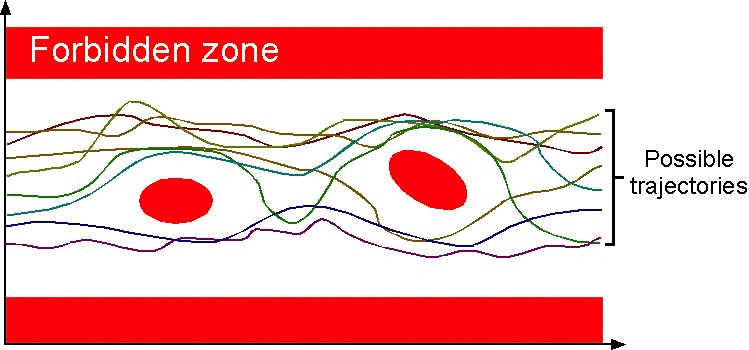
\includegraphics[width=1 \linewidth]{ai-1.png}
        \caption{%
            \emph{Concrete semantics} of programs with
            \emph{forbidden zones}
        }
        \label{fig:ai1}
    \end{subfigure}
%
    \hfill
%
    \begin{subfigure}[hbt]{.45\linewidth}
        \centering
        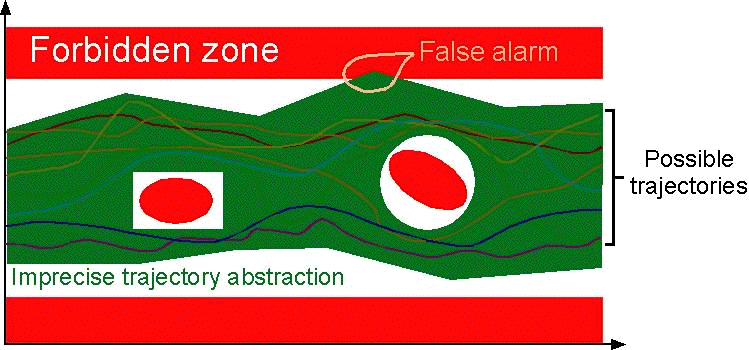
\includegraphics[width=1 \linewidth]{ai-2.png}
        \caption{%
            \emph{Abstract semantics} of programs with imprecise
            trajectory abstraction
        }
        \label{fig:ai2}
    \end{subfigure}

    \caption{%
        Abstract interpretation demonstration~\cite{AIInNutshellCousot}.
        Horizontal axes: time~$ t $. Vertical axes:
        vector~$ x(t) $~of input, state, and output values of the
        considered program
    }
\end{figure}

\subsubsection{Components of Abstract Interpretation}

In accordance with~\cite{savAI, harmimBP}, the basic
components of abstract interpretation are as follows:
\begin{itemize}
    \item
        \textbf{An Abstract Domain}~\cite{AICousotWeb}:

        \begin{itemize}
            \item
                An abstraction of the possible concrete program states
                (or their parts) in the form of \emph{abstract
                properties}\footnote{\textbf{Abstract properties}
                approximating \emph{concrete properties behaviours}.}
                and \emph{abstract operations}\footnote{\textbf{Abstract
                operations} include abstractions of the \emph{concrete
                approximation}, an approximation of the \emph{concrete
                fixpoint transform function},
                etc.}~\cite{AIBasedFormalMethodsCousot}.

            \item
                Sets of program states at certain locations are represented
                using \emph{abstract states}.
        \end{itemize}

    \item
        \textbf{Abstract Transformers}:

        \begin{itemize}
            \item
                There is a~\emph{transform function} for each program
                operation (instruction) that represents the impact
                of the operation executed on an abstract state.
        \end{itemize}

    \item
        \textbf{The Join Operator}~$ \sqcup $:

        \begin{itemize}
            \item
                Joins abstract states from individual program branches into
                a~single one.
        \end{itemize}

    \item
        \textbf{The Widening
        Operator~$ \triangledown $}~\cite{programAnalysisNielson,
        wideningNarrowingCousot, savAI}:

        \begin{itemize}
            \item
                Enforces termination of the abstract interpretation.

            \item
                It is used to approximate the \emph{least fixed points}
                of program semantics (it is performed on a~sequence of
                abstract states at a~certain location).

            \item
                Usually, the later in the analysis this operator is used,
                the more accurate the result is (but the analysis takes more
                time).
        \end{itemize}

    \item
        \textbf{The Narrowing
        Operator~$ \vartriangle $}~\cite{programAnalysisNielson,
        wideningNarrowingCousot, savAI}:

        \begin{itemize}
            \item
                Using this operator, the approximation obtained by
                widening can be refined, i.e., it may be used to refine the
                result of widening.

            \item
                This operator is used when a~\emph{fixpoint} is
                approximated using widening.
        \end{itemize}
\end{itemize}

\subsubsection{Fixpoints and Fixpoint Approximation}

A~\textbf{fixpoint} of a~function  $ f : A \rightarrow A $ is an
element $ a \in A $ if and only if
$ \boldsymbol{f(a) = a} $~\cite{harmimBP}.

Computation of the \emph{most precise abstract fixpoint} is not generally
guaranteed to terminate, in particular, when a~given program contains
a~loop or recursion. The solution is to approximate the fixpoint using
\emph{widening} (over-approximation of a~fixpoint) and \emph{narrowing}
(improves the approximation of the fixpoint)~\cite{savAI,
harmimBP}. Most program properties can be represented as
fixpoints. This reduces program analysis to the fixpoint
approximation~\cite{AICousotWeb}. Further information about fixpoint
approximation can be found, e.g., in~\cite{programAnalysisNielson,
wideningNarrowingCousot}.

\subsubsection{Formal Definition of Abstract Interpretation}

According to~\cite{AILatticeModelCousot, savAI},
\textbf{abstract interpretation}~$ \boldsymbol{I} $~of a~program~$ P $~with
the instruction set~$ S $~is a~tuple
$$ \boldsymbol{I = (Q, \sqcup, \sqsubseteq, \top, \bot, \tau)} $$
where
\begin{itemize}
    \item
        $ \boldsymbol{Q} $~is the \emph{abstract domain} (domain of
        \emph{abstract states}),

    \item
        $ \boldsymbol{\sqcup}~\text{:}~Q \times Q \rightarrow Q $
        is the \emph{join operator} for accumulation of abstract states,

    \item
        $ \text{(}\boldsymbol{\sqsubseteq}\text{)} \subseteq Q \times Q $ is
        an \emph{ordering} defined as
        $ x \sqsubseteq y \Leftrightarrow x \sqcup y = y $ in
        $ (Q, \sqcup, \top) $,

    \item
        $ \boldsymbol{\top} \in Q $ is the \emph{supremum} of~$ Q $,

    \item
        $ \boldsymbol{\bot} \in Q $ is the \emph{infimum} of~$ Q $,

    \item
        $ \boldsymbol{\tau}~\text{:}~S \times Q \rightarrow Q $
        defines \emph{abstract transformers} for specific instructions,

    \item
        $ (Q, \sqcup, \top) $ is a~\emph{complete
        semilattice}~\cite{harmimBP, savAI}.
\end{itemize}

Using so-called \emph{Galois connections}~\cite{programAnalysisNielson,
wideningNarrowingCousot, savAI, AICousotWeb}, one can guarantee the
\emph{soundness} of abstract interpretation.


\section{\texorpdfstring{Facebook Infer\,---\,Static Analysis Framework}{%
    Facebook Infer - Static Analysis Framework%
}}
\label{sec:fbinfer}

\todo{Citovat Vladovu bakalářku. Zmínit se o~C\#.}

This section describes the principles and features of
\emph{Facebook Infer}. The description is based on information provided
at the Facebook Infer website\footnote{\textbf{Facebook Infer}
website\,--\,\url{https://fbinfer.com}.} and in~\cite{inferAISpeech,
harmimBP}. Parts of this section are taken
from the paper~\cite{harmimBP, excel2021Harmim}.

Facebook Infer is an open-source\footnote{\textbf{Open-source repository of
Facebook Infer} on GitHub\,--\,\url{https://github.com/facebook/infer}.}
static analysis \emph{framework}, which is able to discover various kinds of
software bugs of a~given program, with the stress put on \emph{scalability}.
The basic usage of Facebook Infer is illustrated in Figure~\ref{fig:infer}.
A~more detailed explanation of its architecture is shown below. Facebook
Infer is implemented in \emph{OCaml}\footnote{\textbf{OCaml}
website\,--\,\url{https://ocaml.org}.}\,--\,\emph{functional} programming
language, also supporting \emph{imperative} and \emph{object-oriented}
paradigms. Further details about OCaml can be found in~\cite{realWorldOCaml}
or in official documentation\footnote{\textbf{OCaml
documentation}\,--\,\url{http://caml.inria.fr/pub/docs/manual-ocaml}.},
tutorials\footnote{\textbf{OCaml
tutorials}\,--\,\url{https://ocaml.org/learn/tutorials}.}. Facebook Infer was
originally a~standalone tool focused on \emph{sound verification} of the
absence of \emph{memory safety violations}, which was first published in
the well-known paper~\cite{inferBiabduction}.

\begin{figure}[hbt]
    \centering
    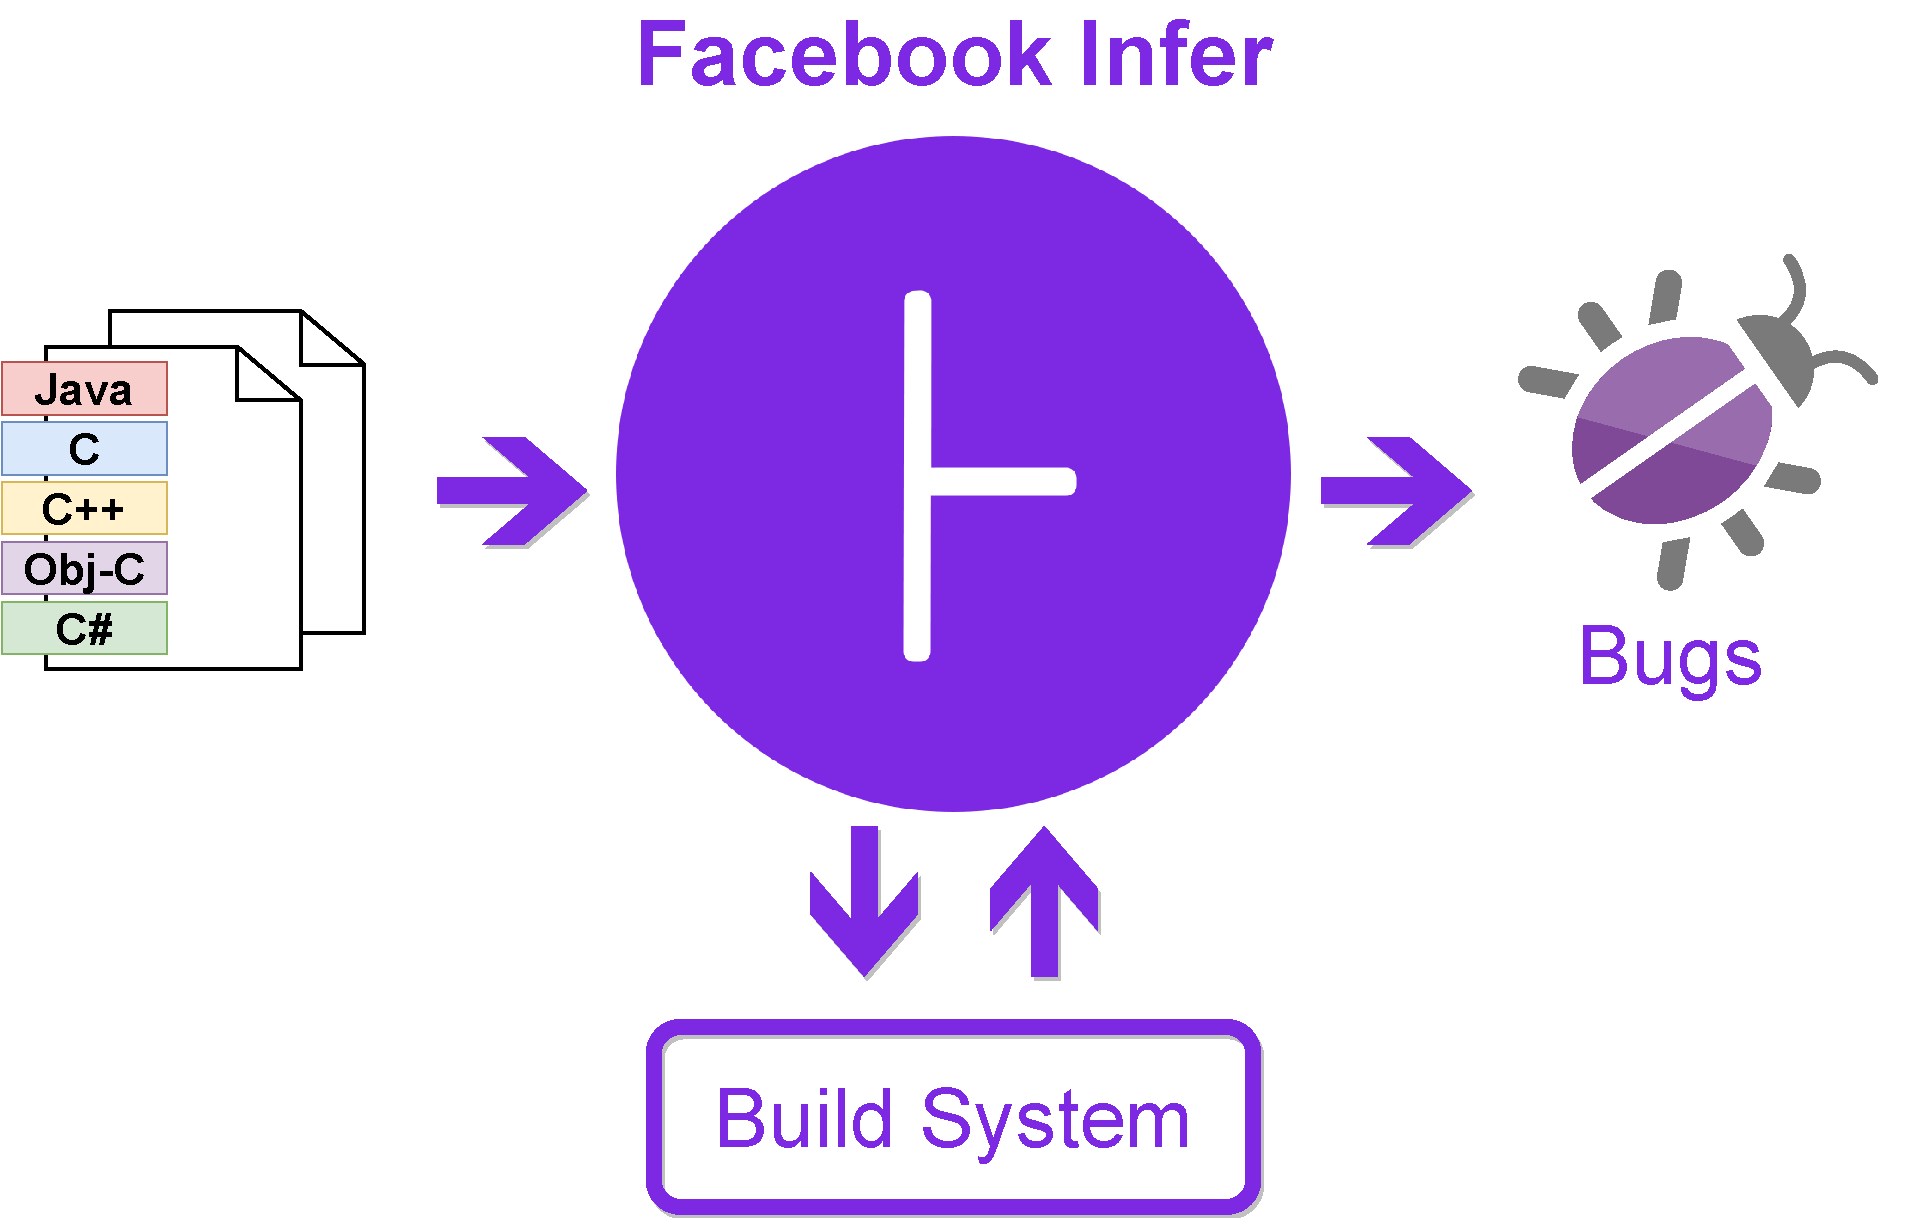
\includegraphics[width=.5 \linewidth]{infer.pdf}
    \caption{%
        Static analysis in Facebook Infer
        (inspired by
        \url{https://adtmag.com/articles/2015/06/12/facebook-infer.aspx})%
    }
    \label{fig:infer}
\end{figure}

Facebook Infer is able to analyse programs written in several languages.
In particular, it supports languages C, C++, Java, and Objective-C. Moreover,
it is possible to extend Facebook Infer's \emph{frontend} for supporting
other languages. Currently, Facebook Infer contains many analyses focusing
on various kinds of bugs, e.g., \emph{Inferbo} (buffer
overruns)~\cite{inferboOnline}; \emph{RacerD} (data races)~\cite{racerD,
racerDOnline, staticRaceDetectorTruePositives}; and other analyses
that check for buffer overflows, some forms of deadlocks and starvation,
null-dereferencing, memory leaks, resource leaks, etc.

\subsection{Abstract Interpretation in Facebook Infer}
\label{sec:fbinferAI}

Facebook Infer is a~general framework for static analysis of programs, it is
based on \emph{abstract interpretation}. Despite the original approach
taken from~\cite{inferBiabduction}, Facebook Infer  aims to find bugs rather
than formal verification. It can be used to quickly develop new sorts of
\emph{compositional} and \emph{incremental} analysers (\emph{intraprocedural}
or \emph{interprocedural}~\cite{programAnalysisNielson}) based
on the concept of function \emph{summaries}. In general, a~\emph{summary}
is a~representation of \emph{preconditions} and \emph{postconditions} of
a~function. However, in practice, a~summary is a~custom data structure that
may be used for storing any information resulting from the analysis of
particular functions. Facebook Infer generally does not compute the summaries
in the course of the analysis along the \emph{Control Flow Graph}
(\textbf{CFG})\footnote{\textbf{A~control flow graph (CFG)} is a~directed
graph in which the nodes represent basic blocks and the edges represent control
flow paths~\cite{controlFlowAnalysisAllen}. \todo{Křena/Vojnar - strana 6, poznámka pod čarou.}} as it is done in classical
analyses based on the concepts from~\cite{DFAGraphReach,
DFAApproaches}. Instead, Facebook Infer performs the
analysis of a~program \emph{function-by-function along the call tree},
starting from its leafs (demonstrated later). Therefore, a~function
is analysed and a~summary is computed without knowledge of the
call context. Then, the summary of a~function is used at all of its call
sites. Since summaries do not differ for different contexts, the analysis
becomes more scalable, but it can lead to a~loss of accuracy. In order
to create a~new intraprocedural analyser in Facebook Infer, it is needed to
define the following (listed items are described in more detail in
Section~\ref{sec:AI}):
\begin{enumerate}
    \item
        The \emph{abstract domain}~$ Q $, i.e., a~type of an
        \emph{abstract state}.

    \item
        Operator~$ \sqsubseteq $, i.e., an \emph{ordering} of abstract
        states.

    \item
        The \emph{join} operator~$ \sqcup $, i.e., the way of joining two
        abstract states.

    \item
        The \emph{widening} operator~$ \triangledown $, i.e., the way how to
        enforce termination of the abstract interpretation of an iteration.

    \item
        \emph{Transfer functions}~$ \tau $, i.e., a~transformer that
        takes an abstract state as an input and produces an abstract state
        as an output.
\end{enumerate}
Further, in order to create an interprocedural analyser, it is required to
additionally define:
\begin{enumerate}
    \item
        The type of function summaries.

    \item
        The logic for using summaries in transfer functions, and the logic
        for transforming an intraprocedural abstract state to
        a~summary.
\end{enumerate}
An important feature of Facebook Infer improving its scalability is
\emph{incrementality} of the analysis, it allows one to analyse separate
code changes only, instead of analysing the whole codebase. It is more
suitable for extensive and variable projects, where ordinary analysis
is not feasible. The incrementality is based on \emph{re-using summaries}
of functions for which there is no change in them neither in the functions
transitively invoked from them.

\subsubsection{%
    The Architecture of the Abstract Interpretation Framework in
    Facebook Infer
}

The architecture of the abstract interpretation framework of Facebook
Infer (\textbf{Infer.AI}) may be split into three major parts,
as demonstrated in Figure~\ref{fig:inferArch}: a~\emph{frontend},
an \emph{analysis scheduler} (and a~\emph{results database}), and a~set of
\emph{analyser plugins}.

The frontend compiles input programs into the \emph{Smallfoot Intermediate
Language} (SIL) and represents them as a~CFG. There is a~separate CFG
representation for each analysed function. Nodes of this CFG are formed as
instructions of SIL. The SIL language consists of the following underlying
instructions:
\begin{itemize}
    \item
        \texttt{LOAD}: reading into a~temporary variable.

    \item
        \texttt{STORE}: writing to a~program variable,
        a~field of a~structure, or an array.

    \item
        \texttt{PRUNE~e}~(often called \texttt{ASSUME}):
        evaluation of a~condition~\texttt{e}.

    \item
        \texttt{CALL}: a~function call.
\end{itemize}
The frontend allows one to propose \emph{language-independent} analyses
(to a~certain extent) because it supports input programs to be written
in multiple languages.

\begin{figure}[hbt]
    \centering
    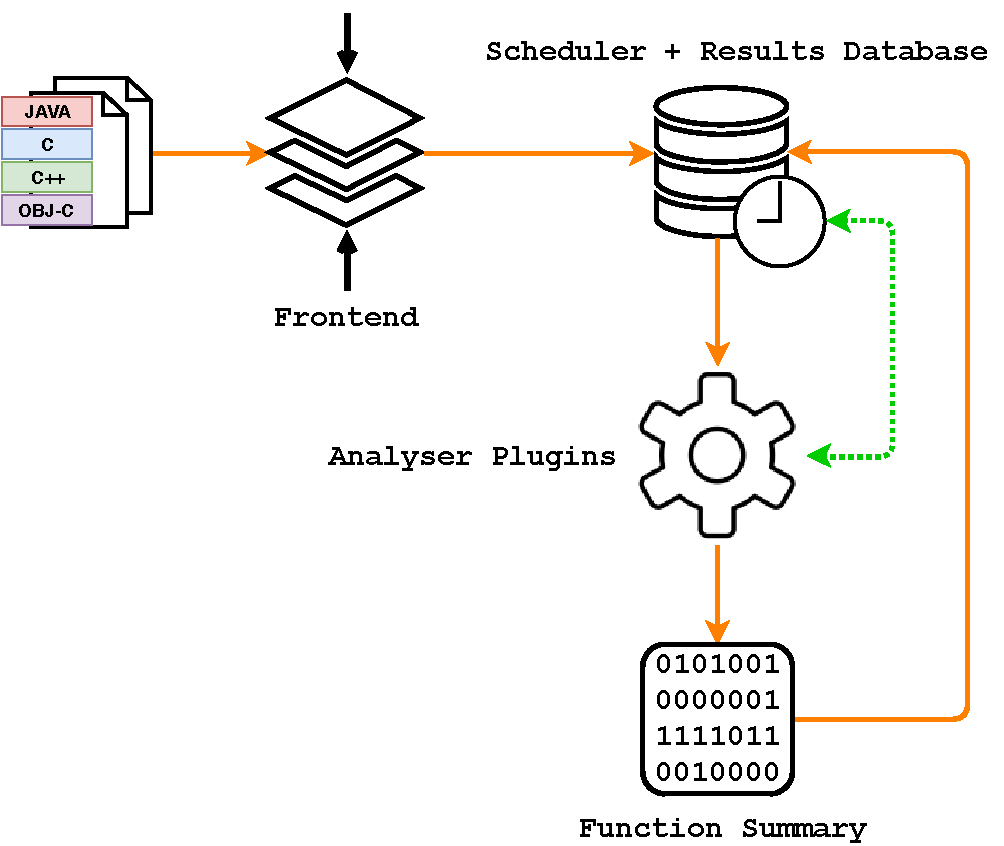
\includegraphics[width=.65 \linewidth]{infer-architecture.pdf}
    \caption{%
        The architecture of Facebook Infer's abstract interpretation
        framework~\cite{inferAISpeech, harmimBP}
    }
    \label{fig:inferArch}
\end{figure}

\begin{wrapfigure}{r}{.45 \linewidth}
    \centering
    \vspace{-1em}
    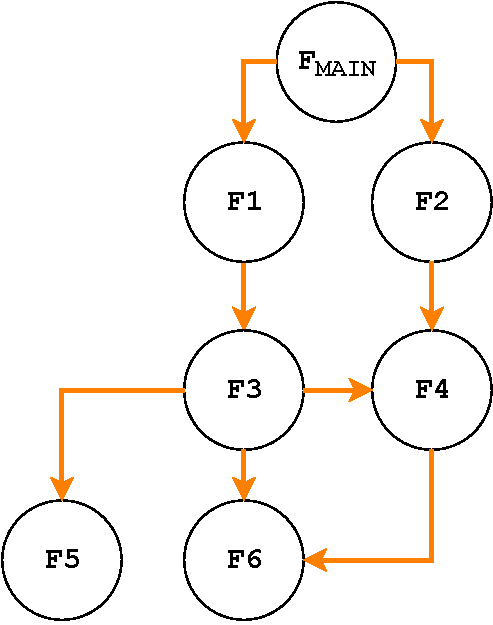
\includegraphics[width=.25 \textwidth]{infer-call-graph.pdf}
    \caption{%
        A~call graph for an illustration of Facebook Infer's
        analysis process~\cite{inferAISpeech, harmimBP}
    }
    \label{fig:inferCallGraph}
\end{wrapfigure}
The next part of the architecture is the scheduler, which defines the
order of the analysis of single functions according to the appropriate
\emph{call graph}\footnote{\textbf{A~call graph} is a~\emph{directed graph}
describing call dependencies among functions.}. The scheduler also checks
if it is possible to analyse some functions simultaneously, which allows
Facebook Infer to run the analysis in parallel.

\begin{example}
    For demonstrating the order of the analysis in Facebook Infer and its
    incrementality, assume a~call graph in Figure~\ref{fig:inferCallGraph}.
    At first, leaf functions \texttt{F5} and \texttt{F6} are analysed.
    Further, the analysis goes on towards the root of the call
    graph\,--\,\texttt{F\textsubscript{MAIN}}, while taking into
    consideration the dependencies denoted by the edges. This order ensures
    that a~summary is available once a~nested function call is abstractly
    interpreted within the analysis. When there is a~subsequent code change,
    only directly changed functions and all the functions up the call path
    are re-analysed. For instance, if there is a~change of source code of
    function \texttt{F4}, Facebook Infer triggers re-analysis of
    functions \texttt{F4}, \texttt{F2}, and \texttt{F\textsubscript{MAIN}}
    only.
\end{example}

The last part of the architecture consists of a~set of analyser plugins.
Each plugin performs some analysis by interpreting of SIL instructions.
The result of the analysis of each function (function summary) is stored to
the results database. The interpretation of SIL instructions (\emph{commands})
is done using an \emph{abstract interpreter} (also called a~\emph{control
interpreter}) and \emph{transfer functions} (also called a~\emph{command
interpreter}). The transfer functions take an actual \emph{abstract state}
of an analysed function as an input, and by applying the interpreting command,
produce a~new abstract state. The abstract interpreter interprets the
command in an \emph{abstract domain} according to the CFG. This workflow is
shown in a~simplified form in Figure~\ref{fig:inferAnalysis}.

\begin{figure}[hbt]
    \centering
    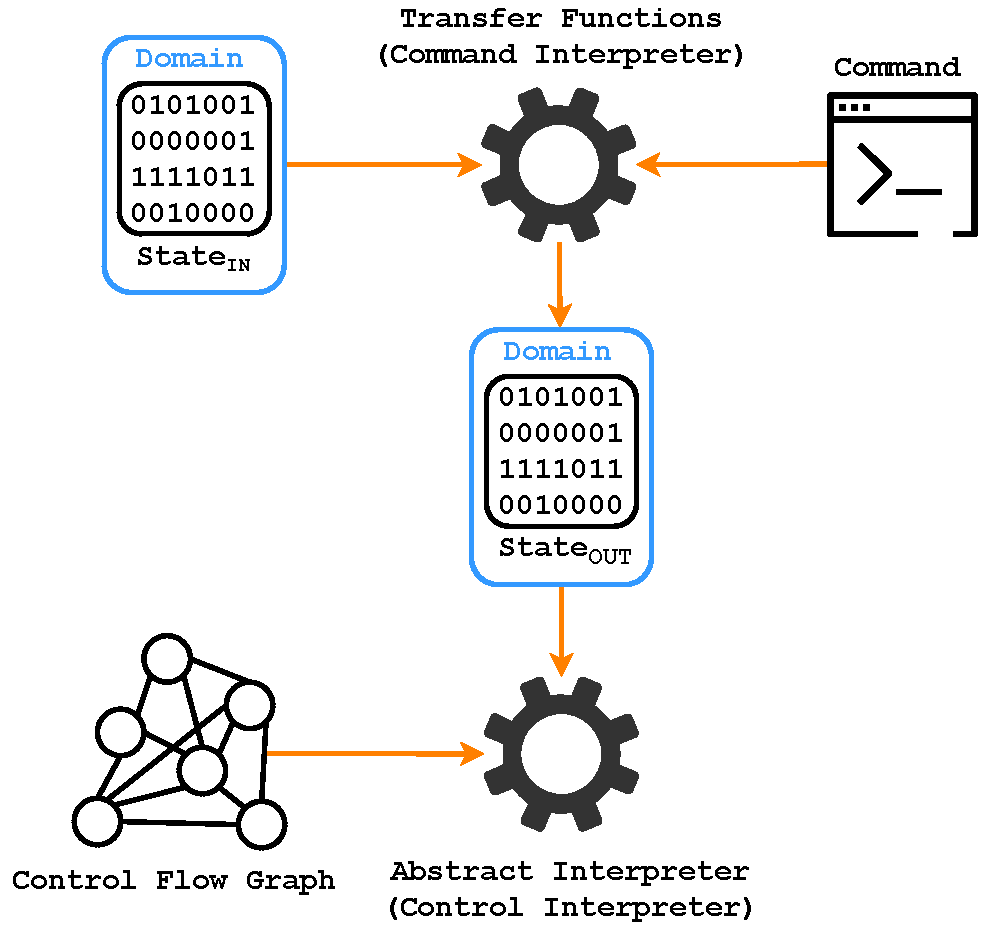
\includegraphics[width=.65 \linewidth]{infer-analysis.pdf}
    \caption{%
        Facebook Infer's abstract interpretation
        process~\cite{inferAISpeech, harmimBP}
    }
    \label{fig:inferAnalysis}
\end{figure}


\section{Contracts for Concurrency}
\label{sec:contracts}

\todo{Přidat něco z~prací Moniky Mužíkovské.}

This section introduces the concept of \emph{contracts for concurrency}
described in~\cite{contracts2015, contracts2017}. Parts of this section are
taken from the thesis~\cite{harmimBP}. Listings in this section are
pieces of programs written in ANSI~C.

Respecting the \emph{protocol} of a~software module\,---\,defines
which \emph{sequences of functions} are legal to invoke\,---\,is one of the
requirements for the correct behaviour of the module. For example, a~module
that deals with a~file system typically requires that a~programmer using
this module should call function \texttt{open} at first, followed by an
optional number of functions \texttt{read} and \texttt{write}, and at last,
call function \texttt{close}. A~program utilising such a~module that does
not follow this protocol is erroneous. The methodology of \emph{design by
contract} (described in~\cite{contract}) requires programs to meet
such well-defined behaviours.~\cite{contracts2015}

In \emph{concurrent programs}, contracts for concurrency allow
one\,---\,in the simplest case\,---\,to specify \emph{sequences of
functions} that are needed to be \emph{executed atomically} in order to
avoid \emph{atomicity violations}. In general, contracts for concurrency
specify sets of sequences of calls that are called \emph{spoilers} and sets
of sequences of calls that are called \emph{targets}, and it is then
required that no target overlaps fully with any spoiler. Such contracts may
be manually specified by a~developer or they may be automatically generated
by a~program (analyser). These contracts can be used to verify the
correctness of programs as well as they can serve as helpful documentation.

Section~\ref{sec:contractsBasic} defines the notion of \emph{basic contracts
for concurrency}. Further, Section~\ref{sec:contractsParams} defines
contracts extended to consider the \emph{data flow} between functions
(where a~sequence of function calls must be atomic only if they handle the
same data). The above mentioned more general contracts for concurrency with
spoilers and targets, which essentially extend the basic contracts with
some \emph{contextual information}, are not presented here in detail
(they are explained in the paper~\cite{contracts2017}). The reason is that
the proposed analyser\,---\,\emph{Atomer}\,---\,so far concentrates on the
basic contracts.

\subsection{Basic Contracts for Concurrency}
\label{sec:contractsBasic}

In~\cite{contracts2017, contracts2015}, a~\emph{basic contract} is
formally defined as follows. Let~$ \Sigma_\mathbb{M} $~be a~set of all
function names of a~software module. A~contract is
a~set~$ \mathbb{R} $~of \emph{clauses} where each clause
$ \varrho\ \in \mathbb{R} $ is a~\emph{star-free regular
expression}\footnote{\textbf{Star-free regular expressions} are
regular expressions using only the \emph{concatenation operators}
and the \emph{alternative operators} ($ | $), without the
\emph{Kleene star operator} ($ * $).} over~$ \Sigma_\mathbb{M} $.
A~\emph{contract violation} occurs if any of the sequences expressed by
the contract clauses are interleaved with the execution of functions
from~$ \Sigma_\mathbb{M} $, in other words, each sequence specified by
any clause~$ \varrho $~must be executed atomically, otherwise, there
is a~violation of the contract. The number of sequences defined by
a~contract is finite since the contract is the union of
\emph{star-free languages}.

\begin{example}
    Consider the following example from~\cite{contracts2017, contracts2015}.
    Assume that there is a~module implementing a~resizable array
    implementing the following interface functions:
    \begin{enumerate}[label={$ f_{\arabic*} $:}]
        \tt

        \item
            \textcolor{bluekeywords}{void} add(%
                \textcolor{bluekeywords}{char} *array,
                \textcolor{bluekeywords}{char} element%
            )

        \item
            \textcolor{bluekeywords}{bool} contains(%
                \textcolor{bluekeywords}{char} *array,
                \textcolor{bluekeywords}{char} element%
            )

        \item
            \textcolor{bluekeywords}{int} index\_of(%
                \textcolor{bluekeywords}{char} *array,
                \textcolor{bluekeywords}{char} element%
            )

        \item
            \textcolor{bluekeywords}{char} get(%
                \textcolor{bluekeywords}{char} *array,
                \textcolor{bluekeywords}{int} index%
            )

        \item
            \textcolor{bluekeywords}{void} set(%
                \textcolor{bluekeywords}{char} *array,
                \textcolor{bluekeywords}{int} index,
                \textcolor{bluekeywords}{char} element%
            )

        \item
            \textcolor{bluekeywords}{void} remove(%
                \textcolor{bluekeywords}{char} *array,
                \textcolor{bluekeywords}{int} index%
            )

        \item
            \textcolor{bluekeywords}{int} size(%
                \textcolor{bluekeywords}{char} *array%
            )
    \end{enumerate}

    The module's contract contains the following clauses:
    \begin{enumerate}[label={$ (\varrho_{\arabic*}) $}]
        \item
            \texttt{contains index\_of}
            \begin{itemize}[label=]
                \item
                    The execution of \texttt{contains} followed by the
                    execution of \texttt{index\_of} should be atomic.
                    Otherwise, the program may fail to get the index,
                    because after verification of the presence of an element
                    in an array, it can be removed by some \emph{concurrently
                    running process}.
            \end{itemize}

        \item
            \texttt{index\_of (get | set | remove)}
            \begin{itemize}[label=]
                \item
                    The execution of \texttt{index\_of} followed by the
                    execution of \texttt{get}, \texttt{set}, or
                    \texttt{remove} should be atomic. Otherwise, the received
                    index may be outdated when it is applied to the address
                    of an element, because a~concurrent modification of an
                    array may shift the position of the element.
            \end{itemize}

        \item
            \texttt{size (get | set | remove)}
            \begin{itemize}[label=]
                \item
                    The execution of \texttt{size} followed by the execution of
                    \texttt{get}, \texttt{set}, or \texttt{remove} should be
                    atomic. Otherwise, the size of an array may be void when
                    accessing an array, because of a~concurrent change of the
                    array. This can be an issue since a~given index is not in
                    a~valid range anymore (e.g., testing
                    \texttt{index < size}).
            \end{itemize}

        \item
            \texttt{add (get | index\_of)}
            \begin{itemize}[label=]
                \item
                    The execution of \texttt{add} followed by the execution of
                    \texttt{get} or \texttt{index\_of} should be atomic.
                    Otherwise, the added element needs no longer exist or its
                    position in an array can be changed, when the program
                    tries to obtain information about it.
            \end{itemize}
    \end{enumerate}
\end{example}

\subsection{Contracts for Concurrency with Parameters}
\label{sec:contractsParams}

The above definition of basic contracts is quite limited in some
circumstances and can consider valid programs as erroneous (reports
\emph{false alarms}). Hence, in this section, there is defined an extension
of basic contracts\,---\,\emph{contracts with parameters}\,---\,which takes
into consideration the data flow within function calls.

\begin{example}
    Consider the following example from~\cite{contracts2017, contracts2015},
    given Listing~\ref{list:contractsReplace}. There is a~function
    \texttt{replace} that replaces item~\texttt{a}~in an array by
    item~\texttt{b}. The implementation of this function comprises two
    atomicity violations:
    \begin{enumerate}[label={(\roman*)}]
        \item
            when \texttt{index\_of} is invoked, item~\texttt{a}~does not
            need to be in the array anymore;

        \item
            the acquired index can be obsolete when \texttt{set} is invoked.
    \end{enumerate}
    A~basic contract could cover this scenario by the clause~$ \varrho_5 $:
    $$ (\varrho_5)\ \text{\texttt{contains index\_of set}} $$
    Nevertheless, this definition is too restrictive because the functions
    are required to be executed atomically only if \texttt{contains} and
    \texttt{index\_of} have the same arguments \texttt{array} and
    \texttt{element}, \texttt{index\_of} and \texttt{set} have the same
    argument \texttt{array}, and the returned value of \texttt{index\_of} is
    used as the argument \texttt{index} of the function \texttt{set}.
\end{example}

\begin{lstlisting}[
    style=c, label={list:contractsReplace}, float=hbt,
    caption={%
        An example of an atomicity violation with data
        dependencies~\cite{contracts2017}
    }
]
void replace(char *array, char a, char b)
{
    if (contains(array, a))
    {
        int index = index_of(array, a);
        set(array, index, b);
    }
}
\end{lstlisting}

In order to respect function call \emph{parameters} and \emph{return values}
of functions in contracts, the basic contracts are extended by
dependencies among functions in~\cite{contracts2017, contracts2015}
as follows. Function call parameters and return values are expressed as
\emph{meta-variables}. Further, if a~contract should be required to be
observed exclusively if the same object emerges as an argument or as the
return value of multiple calls in a~given call sequence, it may be denoted
by using the same meta-variable at the position of all these occurrences of
parameters and return values.

Clause~$ \varrho_5 $~can be extended as follows (repeated application of
meta-variables \texttt{X/Y/Z} requiring the same objects
\texttt{o\textsubscript{1}/o\textsubscript{2}/o\textsubscript{3}} to be used
at the positions of \texttt{X/Y/Z}):
$$
    (\varrho'_5)\ \text{\texttt{%
        contains(X,Y) Z=index\_of(X,Y) set(X,Z,\_)
    }}
$$
The underscore indicates a~\emph{free meta-variable} that does not restrict
the contract clause.

With the extension described above, it is possible to extend the contract
from Section~\ref{sec:contractsBasic} as follows:
\begin{enumerate}[label={$ (\varrho'_{\arabic*}) $}]
    \tt

    \item contains(X,Y) index\_of(X,Y)
    \item Y=index\_of(X,\_) (get(X,Y) | set(X,Y,\_) | remove(X,Y))
\end{enumerate}

\subsection{Contracts for Concurrency with Spoilers}
\label{sec:contractsSpoilers}

\cite{staticRaceDetectorTruePositives}
\cite{inferCSharp}
\cite{contract}
\cite{inferBiabduction}
\cite{controlFlowAnalysisAllen}
\cite{AIBasedFormalMethodsCousot}
\cite{AILatticeModelCousot}
\cite{wideningNarrowingCousot}
\cite{AIInNutshellCousot}
\cite{AICousotWeb}
\cite{inferAISpeech}
\cite{racerDOnline}
\cite{inferboOnline}
\cite{marcinBP}
\cite{DFAGraphReach}
\cite{contracts2015}
\cite{programAnalysisNielson}
\cite{racerD}
\cite{realWorldOCaml}
\cite{deadlockKroening}
\cite{staticAnalysisRival}
\cite{staticAnalysisMoller}
\cite{DFAApproaches}
\cite{savAI}
\cite{hoare}
\cite{anaconda}



%===============================================================================
\chapter{\texorpdfstring{Atomer\,---\,Atomicity Violations Detector}{%
    Atomer - Atomicity Violations Detector%
}}
\label{chap:atomer}

This chapter describes the principles and limitations of the \emph{static
analyser} \emph{Atomer} proposed as a~module of \emph{Facebook Infer}
(introduced in Section~\ref{sec:fbinfer}) for finding some forms of
\emph{atomicity violations}. Atomer was proposed and in detail described in the
bachelor's thesis of the author of this thesis~\cite{harmimBP}. Therefore,
naturally, the following description in Section~\ref{sec:atomerDesing} is based
on the mentioned thesis, and further, there is used information
from~\cite{excel2021Harmim}.

Already existing solutions in this area (besides Atomer)
discusses Section~\ref{sec:atomerRelatedWork}. In particular, it deals with other existing
approaches and tools for finding atomicity violations, their advantages,
disadvantages, features, availability, and so on.

In Section~\ref{sec:atomerLimits}, there are discussed \emph{limitations} and
\emph{shortcomings} of Atomer. Again, some of the thoughts mentioned in this
section are taken into consideration in~\cite{harmimBP, excel2021Harmim}.


\section{Related Work}
\label{sec:atomerRelatedWork}

Atomer is slightly inspired by ideas from~\cite{contracts2017, contracts2015}.
In these papers, there is a~proposal and implementation of a~\emph{static
validation} for finding some forms of \emph{atomicity violations} based on
\emph{grammars} and \emph{parsing trees}. In the paper~\cite{contracts2017},
there is also described and implemented a~\emph{dynamic} approach for the
validation. The authors of these papers implemented a~stand-alone prototype
tool called \emph{Gluon}\footnote{\textbf{Gluon} is a~tool for \emph{static
verification} of \emph{contracts for concurrency}
(see Section~\ref{sec:contracts}) in Java programs. It is available at
\url{https://github.com/trxsys/gluon}.} for analysing programs written in Java.
It led to some promising experimental results, but the \emph{scalability} of
Gluon was still limited.\footnote{Some of the experiments performed by Gluon
are also similarly performed by Atomer, which is mentioned in
Sections~\ref{sec:expGluon} and~\ref{sec:expReal}.} Moreover, Gluon is no more
actively developed. This fact inspired the decision that eventually led to
Atomer, namely, to get inspired by the ideas of~\cite{contracts2017,
contracts2015}, but reimplement them in \emph{Facebook Infer} redesigning it
in accordance with the principles of Facebook Infer (described in
Section~\ref{sec:fbinfer}), which should make the resulting tool more
scalable. In the end, however, due to adapting the analysis for the context
of Facebook Infer, the implementation of the analysis of Atomer is
significantly different from~\cite{contracts2017, contracts2015}, as it is
presented in Chapter~4 of~\cite{harmimBP}. Furthermore,
unlike~\cite{contracts2017, contracts2015}, the implementation aims at
programs written in the \emph{C~language} using \emph{PThread locks} to
\emph{synchronise concurrent threads}.

In Facebook Infer, there was already implemented an analysis called \emph{Lock
Consistency Violation}\footnote{\textbf{Lock Consistency Violation} is an
\emph{atomicity violations} analysis implemented in \emph{Facebook Infer}. It
is described at
\url{https://fbinfer.com/docs/checkers-bug-types/\#lock-consistency-violation}%
.}. It is a~part of \emph{RacerD}~\cite{racerD, staticRaceDetectorTruePositives,
racerDOnline}. This analysis finds atomicity violations in C++ and Objective~C
programs for reads/writes on single variables required to be executed
atomically. Atomer is different; it finds atomicity violations for
\emph{sequences of functions} required to be executed atomically, i.e., it
checks whether \emph{contracts for concurrency}
(see Section~\ref{sec:contracts}) hold. Moreover, it tries to automatically
determine which sequences should indeed be executed atomically (hence, to
\emph{derive the contracts automatically}).


\section{Design of Atomer and Its Principles}
\label{sec:atomerDesing}

\todo{Říct, že Atomer není sound ani complete.}

Atomer concentrates on checking \emph{atomicity of execution of certain
sequences of function calls}, which is often required for \emph{concurrent
programs'} correct behaviour. Atomer's principle is based on the assumption
that sequences of function calls executed \emph{atomically once}
should probably be executed \emph{always atomically}.

Listings in the below sections are pieces of exemplary programs written
in C~language (assuming \emph{POSIX thread}, i.e., \emph{PThread locks}
and declared and initialised global variable \texttt{lock} of a~type
\texttt{phtread\_mutex\_t}).

As it has already been said, the proposal of Atomer is based on the concept
of \emph{contracts for concurrency} described in Section~\ref{sec:contracts}.
In particular, the proposal considers \emph{basic contracts} described in
Section~\ref{sec:contractsBasic}. Neither the contracts extended to
\emph{spoilers} and \emph{targets} (from Section~\ref{sec:contractsSpoilers})
nor contracts extended by \emph{parameters} explained in
Section~\ref{sec:contractsParams} are so far taken into account.

In general, basic contracts for concurrency allow one to define \emph{sequences
of functions} required to be \emph{executed atomically}, as explained in more
detail in Section~\ref{sec:contracts}. Atomer is able to automatically derive
candidates for such contracts and then verify whether the contracts are
fulfilled. Both of these steps are done statically. The proposed analysis is
divided into two parts (\emph{phases of the analysis}):
\begin{enumerate}[label={\textbf{Phase~\arabic*}:}, leftmargin=5em]
    \item
        Detection of (likely) \emph{atomic sequences}.

    \item
        Detection of \emph{atomicity violations} (violations of the atomic
        sequences).
\end{enumerate}
The phases are in-depth described in the sections below. Also, these phases of
the analysis and its workflow are illustrated in
Figure~\ref{fig:atomerPhasesSequences}.

\begin{figure}[hbt]
    \centering
    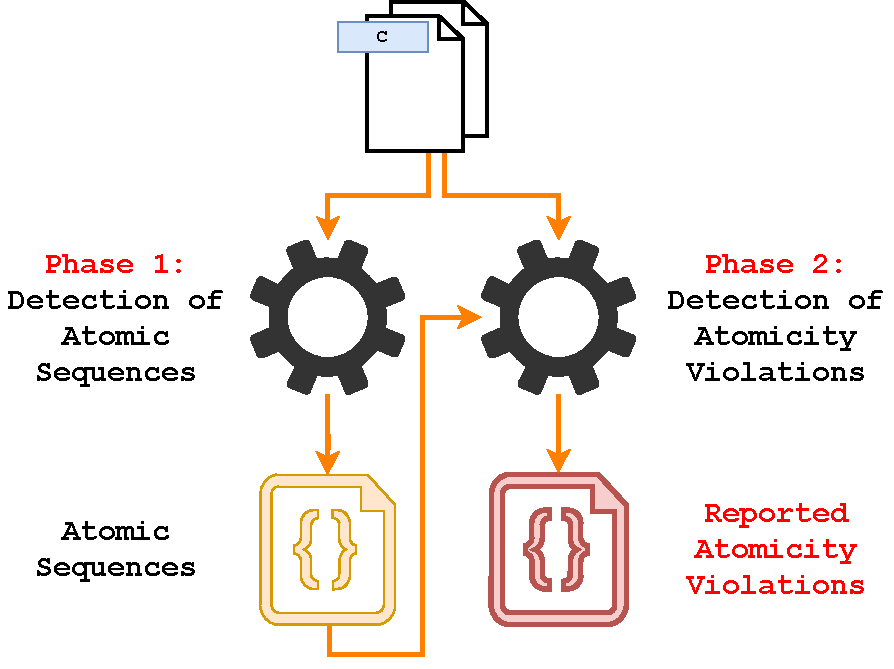
\includegraphics[width=.75 \linewidth]{analyser-proposal.pdf}
    \caption{%
        \emph{Phases} of the Atomer's analysis and the analysis
        \emph{high-level process} illustration%
    }
    \label{fig:atomerPhasesSequences}
\end{figure}

This section describes the proposal of Atomer in general. The concrete types
of the \emph{abstract states} (i.e. elements of the \emph{abstract
domain}~$ \boldsymbol{Q} $) and the \emph{summaries}~$ \chi $, along with the
implementation of all necessary \emph{abstract interpretation operators}
are stated in Chapter~4 of~\cite{harmimBP}. However, actually, the abstract
states~$ s \in \boldsymbol{Q} $ of both phases of the analysis are proposed as
\emph{sets}. So, in fact, the \emph{ordering operator}~$ \sqsubseteq $ is
implemented using testing for a~\emph{subset} (i.e. $ s \sqsubseteq s^\prime
\Leftrightarrow s \subseteq s^\prime $, where $ s, s^\prime \in
\boldsymbol{Q} $), the \emph{join operator}~$ \sqcup $ is implemented as the
\emph{set union} (i.e. $ s \sqcup s^\prime \Leftrightarrow s \cup s^\prime $),
and the \emph{widening operator}~$ \triangledown $ is implemented using the
join operator (i.e. $ s \triangledown s^\prime \Leftrightarrow s \sqcup
s^\prime $).

Function summaries are in below sections reduced to the output parts
(\emph{postconditions}~$ R $) only. The input parts of summaries
(\emph{preconditions}~$ P $) are in case of the proposed analysis always empty,
because, so far, it is not necessary to have any preconditions for analysed
functions. Thus, in this case, the Hoare triple ${ true\ \{Q\}\ R }$ holds,
where~$ Q $ is an analysed program, i.e., $ P = true $.

\subsection{Phase~1: Detection of Atomic Sequences}

Before detecting \emph{atomicity violations} may begin, it is required to have
\emph{contracts} introduced in Section~\ref{sec:contracts}. \textbf{Phase~1}
of Atomer is able to produce such contracts, i.e., it detects \emph{sequences
of functions} that should be \emph{executed atomically}. Intuitively, the
detection is based on looking for sequences of functions executed atomically
on some path through a~program. The assumption is that if it is \emph{once
needed to execute a~sequence atomically}, it should probably be \emph{always
executed atomically}.

For a~description of the analysis, it is first needed to introduce a~notion
of a~\emph{reduced sequence} of function calls. Such a~sequence denotes
a~sequence in which the first appearance of each function is recorded only.
The reason is to ensure the \emph{finiteness} of the sequences derived by the
analysis, and hence the analysis's \emph{termination}. The detection of
sequences of calls to be executed atomically is based on analysing all paths
through the CFG of a~function and generating all pairs $ {(A, B)} \in
{\Sigma^* \times \Sigma^*} $ (where~$ \Sigma^* $ is a~set of all possible
sequences of functions from~$ \Sigma $ from a~given program) of reduced
sequences of function calls for each path such
that: Here, $ A $ is a~reduced sequence of function calls that appear between
the beginning of the function being analysed and the first lock, between an
unlock and a~subsequent lock, or between an unlock and the end of the function
being analysed. $ B $ is a~reduced sequence of function calls that follow the
calls from~$ A $, and that appear between a~lock and an unlock (or between
a~lock and the end of the function being analysed). Thus, the \emph{abstract
state} $ s \in \boldsymbol{Q} $ is defined as $ 2^{2^{\Sigma^* \times
\Sigma^*}} $ (because there is a~set of the ${ (A, B) }$ pairs for each program
path).

It would be more precise to generate longer sequences of type ${ A_1 B_1 A_2
B_2 \ldots }$, instead of the sets of the pairs ${ (A, B) }$. Nevertheless,
it would be more challenging to ensure the above longer sequences' finiteness
and the sets of these sequences' finiteness. Moreover, there would be
a~significantly larger \emph{state space explosion problem}~\cite{stateExpl}.
So, the proposed representation of the sets of pairs of sequences has been
chosen to compromise accuracy and efficiency. However, the experiments
described in Chapter~5 of~\cite{harmimBP} show that it needs even more
pronounced abstraction for appropriate \emph{scalability}.

Formally, the \emph{initial abstract state} of a~function is defined as
$ s_{init} = {\{\{(\varepsilon, \varepsilon)\}\}} $, where~$\varepsilon $
indicates an empty sequence. To formalise the analysis of a~function,
let~\texttt{f} be a~called leaf function. Further, let~$ s_\mathtt{g} $ be the
abstract state of a~function~\texttt{g} being analysed before the
function~\texttt{f} is called. After the call of~\texttt{f}, the abstract state
will be changed as follows: $ s_\mathtt{g} = \{p^\prime \in 2^{\Sigma^* \times
\Sigma^*}\ |\ \exists\,p \in s_\mathtt{g} : p^\prime =
\textcolor{blue}{\{}{(A^\prime, B^\prime)} \in \Sigma^* \times \Sigma^*\ |\
\exists\,{(A, B)} \in p : \textcolor{violet}{(}\neg actual(p, (A, B)) \wedge
{(A^\prime, B^\prime)} = {(A, B)}\textcolor{violet}{)} \vee
\textcolor{red}{[}{actual(p, {(A, B)})} \wedge \textcolor{green}{[}(lock
\wedge {(A^\prime, B^\prime)} = {(A, B \cdot \mathtt{f})}) \vee (\neg lock
\wedge {(A^\prime, B^\prime)} = {(A \cdot \mathtt{f},
B)})\textcolor{green}{]}\textcolor{red}{]}\textcolor{blue}{\}}\} $,
where $ actual $ is a~Boolean function that determines whether a~given
${ (A, B) }$ pair is the most recent pair of sequences of the current program
state for a~given program path. Furthermore, $ lock $ is a~predicate indicating
whether the current program state is inside an atomic block. Furthermore,
let~$ s_\mathtt{g} $ be the abstract state of a~function~\texttt{g} being
analysed before an unlock is called. After the unlock is called, a~new ${ (A,
B) }$ pair is created and labelled as an actual using the function
$ setActual $ as follows: $ s_\mathtt{g} = \{p^\prime \in 2^{\Sigma^*
\times \Sigma^*}\ |\ \exists\,p \in s_\mathtt{g} : p^\prime =
\textcolor{blue}{\{}{(A^\prime, B^\prime)} \in \Sigma^* \times \Sigma^*\
|\ \textcolor{violet}{(}{(A^\prime, B^\prime)} = {(\varepsilon, \varepsilon)}
\wedge setActual(p, {(A^\prime, B^\prime)})\textcolor{violet}{)} \vee
{(A^\prime, B^\prime)} \in p\textcolor{blue}{\}}\} $.

\begin{example}
    For an explanation of the computation of the sets of the pairs ${ (A,
    B) }$, assume that a~state of the analysis of a~program~$ Q $ is the
    following sequence of function calls: \texttt{f,~g}; and a~state of the
    analysis of a~program~$ Q^\prime $ is the following sequence of function
    calls: \texttt{f,~g~[m,~n}. The square brackets are used to indicate an
    \emph{atomic sequence} (the closing square bracket is missing in the case
    of the program~$ Q^\prime $, which means that the program state is
    currently inside an \emph{atomic block}). The computed abstract state for
    the program~$ Q $ is $ s_Q = {\{\{((\mathtt{f, g}), \varepsilon)\}\}} $,
    and for the program~$ Q^\prime $,
    it is $ s_{Q^\prime} = {\{\{((\mathtt{f, g}), (\mathtt{m, n}))\}\}} $. Now,
    if the next instruction is a~call of a~function~\texttt{x}, in the case of
    the program~$ Q $, the call will be added to the first~$ A $ sequence, and
    in the case of the program~$ Q^\prime $, the call will be added to the
    first~$ B $ sequence as follows: $ s_Q = {\{\{((\mathtt{f, g, x}),
    \varepsilon)\}\}} $, $ s_{Q^\prime} = {\{\{((\mathtt{f, g}), (\mathtt{m, n,
    x}))\}\}} $. Subsequently, if the next step in the program~$ Q $ is a~lock
    call, the next function calls will be added to the first~$ B $ sequence
    of the set~$ s_Q $. And if the next step in the program~$ Q^\prime $ is an
    unlock call, it will be created a~new element of the first set of the
    set~$ s_{Q^\prime} $, and the next function calls will be added to
    the~$ A $ sequence of this element. Finally, if a~function~\texttt{y} is
    called, the resulting sets will look like follows: $ s_Q =
    {\{\{((\mathtt{f, g, x}), (\mathtt{y}))\}\}} $, $ s_{Q^\prime} =
    {\{\{((\mathtt{f, g}), (\mathtt{m, n, x})), ((\mathtt{y}),\
    \varepsilon)\}\}} $. Note that the final sequences of function calls
    look like follows: \texttt{f,~g,~x~[y} and \texttt{f,~g~[m,~n,~x]~y} for
    the programs~$ Q $, and~$ Q^\prime $, respectively.
\end{example}

The \emph{summary}~$ \chi_\mathtt{f} \in 2^{\Sigma^*} \times \Sigma^* $ of
a~function~\texttt{f} is then defined as $ \chi_\mathtt{f} = (\boldsymbol{B},
AB) $, where:
\begin{itemize}
    \item
        $ \boldsymbol{B} $ is a~set constructed that contains all the~$ B $
        sequences that appear on program paths through~\texttt{f}, i.e.,
        $ \boldsymbol{B} = \{B^\prime \in \Sigma^*\ |\ \exists\,p \in
        s_\mathtt{f} : \exists\,{(A, B)} \in p : B \neq \varepsilon \wedge
        B^\prime = B\} $, where~$ s_\mathtt{f} $ is the abstract state at the
        end of an interpretation of~\texttt{f}. In other words, this component
        of the summary is a~set of sequences of atomic function calls appearing
        in an analysed function.

    \item
        $ AB $ is a~\emph{concatenation} of all the~$ A $ and~$ B $
        sequences with removed duplicates of function calls. In particular,
        assume that there is the following computed set of ${ (A, B) }$
        pairs: $ \{{(A_1, B_1)}, {(A_2, B_2)}, \ldots, {(A_n, B_n)}\} $,
        then the result is concatenated sequence ${ A_1 \cdot B_1 \cdot A_2
        \cdot B_2 \cdot \ldots \cdot A_n \cdot B_n }$ with removed
        duplicates. Formally:
        $$
            AB = reduce(\bigcup\limits_{ab \in AB^\prime}^\cdot ab)
        $$
        where $ AB^\prime = \{ab \in \Sigma^*\ |\ \exists\,p \in s_\mathtt{f}
        : \exists\,(A, B) \in p: ab = {A \cdot B}\} $, $ reduce $ is a~function
        that removes duplicates of function calls, and $ \dot\bigcup $
        concatenates all sequences of a~set. Intuitively, in this component
        of the summary, it is gathered  occurrences of all called functions
        within an analysed function obtained by concatenation of all
        the~$ A $ and~$ B $ sequences.
\end{itemize}
$ AB $ is recorded to analyse functions higher in the \emph{call hierarchy}
since locks/unlocks can appear in such a~\emph{higher-level} function.

\begin{example}
    For instance, the analysis of the function~\texttt{f} from
    Listing~\ref{list:atomerPhase1} produces the following sequences:
    $$
        \overbrace{\text{\texttt{a,~\sout{a}}}}^{A_1}~%
        \overbrace{\text{\texttt{[a,~\sout{a},~b]}}}^{B_1}~%
        \overbrace{\text{\texttt{a,~\sout{a}}}}^{A_2}~%
        \overbrace{\text{\texttt{[a,~c]}}}^{B_2}~%
        \text{\sout{\ensuremath{%
            \overbrace{\text{\texttt{a}}}^{\text{\sout{\ensuremath{A_3}}}}~%
            \overbrace{\text{\texttt{[a,~c,~c]}}}%
            ^{\text{\sout{\ensuremath{B_3}}}}%
        }}}
    $$
    The functions~\texttt{a, b, c} are not deeper analysed because it
    is assumed that these functions are leaf nodes of the \emph{call
    graph}. The strikethrough of the functions~\texttt{a} and~\texttt{c}
    denotes removing already recorded function calls in the~$ A $
    and~$ B $ sequences. The strikethrough of the entire sequence
    \texttt{a~[a,~c,~c]} means discarding sequence already seen before.
    For the above, the abstract state at the end of an interpretation
    of the function~\texttt{f} is $ s_\mathtt{f} = \{\{{((\mathtt{a}),
    (\mathtt{a, b}))}, {((\mathtt{a}), (\mathtt{a, c}))}, {(\varepsilon,
    \varepsilon)}\}\} $. The derived summary~$ \chi_\mathtt{f} $ for the
    function~\texttt{f} is $ \chi_\mathtt{f} = {(\boldsymbol{B}, AB)} $,
    where:
    \begin{itemize}
        \item
            $ \boldsymbol{B} = \{{(\mathtt{a, b})}, {(\mathtt{a, c})}\} $,
            i.e., $ B_1 $ and~$ B_2 $;

        \item
            $ AB = {(\mathtt{a, b, c})} $, i.e., the concatenation
            of~$ A_1 $, $ B_1 $, $ A_2 $, and $ B_2 $ from which
            duplicate function calls were removed.
    \end{itemize}
\end{example}

\begin{lstlisting}[
    style=c, label={list:atomerPhase1}, float=hbt,
    caption={%
        A~code snippet used for an illustration of the derivation of
        \emph{sequences of functions called atomically}%
    }
]
void f()
{
    a(); a();

    <@\textcolor{red}{pthread\_mutex\_lock}@>(&lock); // (a, b)
    a(); a(); b();
    <@\textcolor{red}{pthread\_mutex\_unlock}@>(&lock);

    a(); a();

    <@\textcolor{red}{pthread\_mutex\_lock}@>(&lock); // (a, c)
    a(); c();
    <@\textcolor{red}{pthread\_mutex\_unlock}@>(&lock);

    a();

    <@\textcolor{red}{pthread\_mutex\_lock}@>(&lock); // (a, c)
    a(); c(); c();
    <@\textcolor{red}{pthread\_mutex\_unlock}@>(&lock);
}
\end{lstlisting}

Further, it is demonstrated how the results of the analysis of \emph{nested
functions} are used during the detection of atomic sequences. The result of
the analysis of a~nested function is used as follows. When calling an already
analysed function, one plugs the sequences from the second component of its
summary (i.e. the $ AB $ sequence) into the most recent~$ A $ or~$ B $
sequence of all the program paths (where a~program path corresponds to
a~single element of an abstract state, i.e., a~set of the ${ (A, B) }$
pairs). In particular, assume that ${ (A, B) }$ is the most recent pair
of sequences of the program state of a~path being analysed. Subsequently, it
is called a~function~\texttt{f} with a~\emph{non-empty summary} (i.e. $ AB
\neq \varepsilon $). If the current program state of an analysed function is
inside an atomic block, the analysis in this step will transform the
pair~${ (A, B) }$ to a~new ${ (A^\prime, B^\prime) }$ pair as follows:
$ {(A^\prime, B^\prime)} = {(A, B \cdot \mathtt{f} \cdot AB)} $. Otherwise,
$ {(A^\prime, B^\prime)} = {(A \cdot \mathtt{f} \cdot AB, B)} $. In such cases
where a~summary is empty, i.e., there are no function calls in a~called
function, or it is a~leaf node of the call graph, it is appended just the
function name to the most recent~$ A $ or~$ B $ sequences of all the program
paths. To formalise this process, let~\texttt{f} be a~called function that was
already analysed, and the second component of its summary is $ AB $. Further,
let~$ s_\mathtt{g} $ be the abstract state of a~function~\texttt{g} being
analysed before the function~\texttt{f} is called. After the call of~\texttt{f},
the abstract state will be changed as follows: $ s_\mathtt{g} = \{p^\prime \in
2^{\Sigma^* \times \Sigma^*}\ |\ \exists\,p \in s_\mathtt{g} : p^\prime =
\textcolor{blue}{\{}{(A^\prime, B^\prime)} \in \Sigma^* \times \Sigma^*\ |\
\exists\,{(A, B)} \in p : \textcolor{violet}{(}\neg actual(p, (A, B)) \wedge
{(A^\prime, B^\prime)} = {(A, B)}\textcolor{violet}{)} \vee
\textcolor{red}{[}{actual(p, {(A, B)})} \wedge \textcolor{green}{[}(lock
\wedge {(A^\prime, B^\prime)} = {(A, B \cdot \mathtt{f} \cdot AB)}) \vee
(\neg lock \wedge {(A^\prime, B^\prime)} = {(A \cdot \mathtt{f} \cdot AB,
B)})\textcolor{green}{]}\textcolor{red}{]}\textcolor{blue}{\}}\} $.

\begin{example}
    This example shows how the function~\texttt{g} from
    Listing~\ref{list:atomerPhase1Nested} would be analysed using the result
    of the analysis of the function~\texttt{f}
    from Listing~\ref{list:atomerPhase1}. So the analysis of the
    function~\texttt{g} produces the following sequence:
    $$
        \text{\texttt{a,~f,~\sout{a},~b,~c}}~%
        \text{\texttt{[f,~a,~b,~c]}}
    $$
    For the above, the abstract state at the end of an interpretation of the
    function~\texttt{g} is $ s_\mathtt{g} = \{\{({(\mathtt{a,~f,~b,~c})},
    {(\mathtt{f,~a,~b,~c})}), {(\varepsilon, \varepsilon)}\}\} $. The derived
    summary~$ \chi_\mathtt{g} $ for the function~\texttt{g} is $
    \chi_\mathtt{g} = ({\{(\mathtt{f,~a,~b,~c})\}},
    {(\mathtt{a,~f,~b,~c})}) $.
\end{example}

\begin{lstlisting}[
    style=c, label={list:atomerPhase1Nested}, float=hbt,
    caption={%
        A~code snippet used to illustrate the derivation of
        \emph{sequences of functions called atomically} with a~\emph{nested
        function calls} (function~\texttt{f} is defined in
        Listing~\ref{list:atomerPhase1})%
    }
]
void g()
{
    a(); f();

    <@\textcolor{red}{pthread\_mutex\_lock}@>(&lock); // (f, a, b, c)
    f();
    <@\textcolor{red}{pthread\_mutex\_unlock}@>(&lock);
}
\end{lstlisting}

\paragraph{Cases Where Lock/Unlock Calls Are Not Paired in a~Function}

For treating cases where \emph{lock/unlock calls are not paired} in
a~function\,---\,as demonstrated in
Listing~\ref{list:AtomerPhase1NotPairedLock}\,---\,in Atomer, the
following solution is implemented.

\emph{Everything is unlocked} at the end of a~function, i.e.,
one \emph{virtually} appends an unlock to the end of the function if it is
necessary. Then, for the function~\texttt{x} from
Listing~\ref{list:AtomerPhase1NotPairedLock}, the atomic section is
virtually closed. Hence, there is detected an atomic sequence
$ (\mathtt{a}) $. In particular, the summary is as follows:
$ \chi_\mathtt{x} = (\{(\mathtt{a})\}, (\mathtt{a})) $.

Moreover, \emph{all unlock calls not preceded by a~lock are ignored}.
Thus, in the function~\texttt{y} from
Listing~\ref{list:AtomerPhase1NotPairedLock}, there are not detected
any atomic sequences: $ \chi_\mathtt{y} = (\emptyset, (\mathtt{a})) $.

\begin{lstlisting}[
    style=c, label={list:AtomerPhase1NotPairedLock}, float=hbt,
    caption={%
        A~code snippet used to illustrate treating cases where
        \emph{lock/unlock calls are not paired} in a~function%
    }
]
void x()
{
    <@\textcolor{red}{pthread\_mutex\_lock}@>(&lock); // (a)
    a();
}
void y()
{
    a();
    <@\textcolor{red}{pthread\_mutex\_unlock}@>(&lock);
}
\end{lstlisting}

\paragraph{Summary of the Phase~1}

The above detection of atomic sequences was implemented and also validated
on a~set of sample programs created for testing purposes, which is described
in~\cite{harmimBP}. The derived sequences of calls assumed to execute
atomically\,---\,the~$ \boldsymbol{B} $ sequences\,---\,from the summaries
of all analysed functions are stored into a~file used during \textbf{Phase~2},
which is described below.

\subsection{Phase~2: Detection of Atomicity Violations}

In the second phase of the analysis, i.e., when \emph{detecting violations}
of the atomic sequences obtained from \textbf{Phase~1}, the analysis looks
for \emph{pairs of functions} that \emph{should be called atomically} (or
just for single functions if there is only one function call in an atomic
sequence) while this is not the case on some path through the CFG. The
pairs of function calls to be checked for atomicity are obtained as
follows: For each function~\texttt{f} with the
\emph{summary}~$ \chi_\mathtt{f} = {(\boldsymbol{B}, AB)} $ in a~given
program~$ Q $, it is taken the first component~$ \boldsymbol{B} $ of the
summary~$ \chi_\mathtt{f} $, i.e., $ \boldsymbol{B} = {\{B_1, B_2,
\ldots, B_n\}} $, and it is taken \emph{every pair} $ {(\mathtt{x},
\mathtt{y})} \in \Sigma \times \Sigma $ of functions that appear as
a~\emph{substring} in some of the~$ B_i $ sequences, i.e., $ B_i = w \cdot
\mathtt{x} \cdot \mathtt{y} \cdot w^\prime $ for some sequences~$ w,
w^\prime $. Note that~\texttt{x} could be~$ \varepsilon $ (an empty
sequence) if some~$ B_i $ consists of a~single function. All these
\uv{atomic pairs} are put into the set $ \Omega \in 2^{\Sigma \times
\Sigma} $. More formally, $ \Omega = \{(\mathtt{x}, \mathtt{y}) \in
\Sigma \times \Sigma\ |\ \exists\,{(\boldsymbol{B}, AB)} \in X_Q :
\exists\,B \in \boldsymbol{B} : (|B| = 1 \wedge {(\mathtt{x}, \mathtt{y})}
= {(\varepsilon, B)}) \vee (|B| > 1 \wedge \exists\,w, w^\prime \in
\Sigma^* : B = w \cdot \mathtt{x} \cdot \mathtt{y} \cdot w^\prime \wedge
{(\mathtt{x}, \mathtt{y})} \neq {(\varepsilon, \varepsilon)})\} $,
where~$ \Sigma^* $ is a~set of all possible sequences of functions
from~$ \Sigma $ from a~given program, and $ X_Q \in 2^{2^{\Sigma^*}
\times \Sigma^*} $ is a~set of all summaries of the program~$ Q $.

\begin{example}
    For instance, assume that in \textbf{Phase~1}, there was analysed
    a~function~\texttt{f}. Which produced the summary
    $ \chi_\mathtt{f} = (\boldsymbol{B}, AB) $, where
    $ \boldsymbol{B} = \{{(\mathtt{a}, \mathtt{b}, \mathtt{c})},
    {(\mathtt{a}, \mathtt{c}, \mathtt{d})\}} $, i.e., a~set of
    sequences of functions that should be called atomically. The
    analysis will then look for the following pairs of functions that
    are not called atomically: $ \Omega = \{{(\mathtt{a}, \mathtt{b})},
    {(\mathtt{b}, \mathtt{c})}, {(\mathtt{a}, \mathtt{c})},
    {(\mathtt{c}, \mathtt{d})}\} $.
\end{example}

An element of this phase's \emph{abstract state} is a~triple
$ {(\mathtt{x}, \mathtt{y}, \Delta)} \in \Sigma \times \Sigma \times
2^{\Sigma \times \Sigma} $, where $ {(\mathtt{x}, \mathtt{y})} $ is
a~pair of the most recent function calls, and~$ \Delta $ is
a~\emph{set of pairs that violate atomicity}. Thus, the abstract
state $ s \in \boldsymbol{Q} $ is defined as $ 2^{\Sigma \times \Sigma
\times 2^{\Sigma \times \Sigma}} $. Whenever a~function~\texttt{f} is
called, it is created a~new pair ${ (\mathtt{x}^\prime,
\mathtt{y}^\prime) }$ of the most recent function calls from the
previous pair ${ (\mathtt{x}, \mathtt{y}) }$ (i.e. $ {(\mathtt{x}^\prime,
\mathtt{y}^\prime)} = {(\mathtt{y}, \mathtt{f})} $). Further, when the
current program state is not inside an atomic block, it is checked
whether the new pair (or just the last call) violates atomicity (i.e.
$ {(\mathtt{x}^\prime, \mathtt{y}^\prime)} \in \Omega \vee
{(\varepsilon, \mathtt{y}^\prime)} \in \Omega $). When it does,
it is added to the set~$ \Delta $ of pairs that violate atomicity.

Formally, the \emph{initial abstract state} of a~function is defined as
$ s_{init} = {\{(\varepsilon, \varepsilon, \emptyset)\}} $.
To formalise the analysis of a~function, let~\texttt{f} be a~called leaf
function. Further, let~$ s_\mathtt{g} $ be the abstract state of
a~function~\texttt{g} being analysed before the function~\texttt{f} is
called. After the call of~\texttt{f}, the abstract state will be
changed as follows: $ s_\mathtt{g} = \{{(\mathtt{x}^\prime,
\mathtt{y}^\prime, \Delta^\prime)} \in \Sigma \times \Sigma \times
2^{\Sigma \times \Sigma}\ |\ \exists\,{(\mathtt{x}, \mathtt{y}, \Delta)}
\in s_\mathtt{g} : {(\mathtt{x}^\prime, \mathtt{y}^\prime)} = {(\mathtt{y},
\mathtt{f})} \wedge \textcolor{orange}{[}\textcolor{green}{(}\neg lock
\wedge \Delta^\prime = \textcolor{red}{\{}{(\mathtt{x}^{\prime\prime},
\mathtt{y}^{\prime\prime})} \in \Sigma \times \Sigma\ |\
{(\mathtt{x}^{\prime\prime}, \mathtt{y}^{\prime\prime})} \in \Delta \vee
[\textcolor{violet}{(}{(\mathtt{x}^{\prime\prime},
\mathtt{y}^{\prime\prime})} = {(\mathtt{x}^{\prime}, \mathtt{y}^\prime)}
\vee {(\mathtt{x}^{\prime\prime}, \mathtt{y}^{\prime\prime})} =
{(\varepsilon, \mathtt{y}^\prime)}\textcolor{violet}{)} \wedge
{(\mathtt{x}^{\prime\prime}, \mathtt{y}^{\prime\prime})} \in
\Omega]\textcolor{red}{\}}\textcolor{green}{)} \vee (lock
\wedge \Delta^\prime = \Delta)\textcolor{orange}{]}\} $.

The analysis of functions with \emph{nested function calls} and cases
where \emph{lock/unlock calls not not paired} in functions are
handled analogically as in \textbf{Phase~1}. For detailed examples,
see~\cite{harmimBP}.

\begin{example}
    To demonstrate the detection of an atomicity violation,
    assume the functions~\texttt{f} and~\texttt{g} from
    Listing~\ref{list:AtomerPhase2}. The set of atomic sequences
    of the function~\texttt{f} with the summary~$ \chi_\mathtt{f}
    = (\boldsymbol{B}, AB) $ is $ \boldsymbol{B} = {\{(\mathtt{b},
    \mathtt{c})\}} $, thus $ \Omega = {\{(\mathtt{b}, \mathtt{c})\}} $.
    In the function~\texttt{g}, an atomicity violation is detected
    because the pair of functions~\texttt{b} and~\texttt{c} is not
    called atomically (under a~lock).
\end{example}

\begin{lstlisting}[
    style=c, label={list:AtomerPhase2}, float=hbt,
    caption={Example of an \emph{atomicity violation}}
]
void f()
{
    a();

    <@\textcolor{red}{pthread\_mutex\_lock}@>(&lock); // (b, c)
    b(); c();
    <@\textcolor{red}{pthread\_mutex\_unlock}@>(&lock);

    d();
}
void g()
{
    a(); b(); c(); d(); // <@\textcolor{red}{ATOMICITY\_VIOLATION:}@> (b, c)
}
\end{lstlisting}

\paragraph{Summary of the Phase~2}

Like in the first phase of the analysis, \textbf{Phase~2} was implemented
and validated on a~set of purposeful sample programs, as it is described
in~\cite{harmimBP}. The sets of atomicity violations~$ \Delta $ from individual
functions are the final reported atomicity violations seen by a~user.


\section{Atomer's Limitations}
\label{sec:atomerLimits}

Atomer was proposed as it is detailed in Section~\ref{sec:atomerDesing}. The
analyser was implemented, and it is working as expected. Moreover, it can
be used in practice to analyse various kinds of programs, and it may find
\emph{real atomicity related bugs}. Nevertheless, there are still several
limitations and cases where Atomer would not work correctly, i.e., cases not
considered during the original proposal. Some of these cases were briefly
discussed in~\cite{harmimBP}, and further described in~\cite{excel2021Harmim}.

So far, Atomer does not work with \emph{nested locks}, i.e., it does not
distinguish \emph{different locks} used in a~program. Only calls of
locks/unlocks are identified, and parameters of these calls (\emph{lock
objects}) are not considered. So, if there are several lock objects used, the
analysis does not work correctly. Although this may happen in \emph{real-life
programs}, insomuch as one could have another (smaller) atomic section inside
a~current atomic section (this does not have to be evident at first because
the \emph{inner atomic section} could be, e.g., included via a~macro). For
instance: \texttt{lock(A); lock(B); \ldots\ unlock(B); unlock(A);}. Another
possibility is an \emph{alternating sequence of locks}, e.g., two locks are
locked at first, and then, they are unlocked in the same order, i.e.,
\texttt{lock(A); lock(B); \ldots\ unlock(A); unlock(B);}.

Atomer considers only \emph{basic contracts for concurrency}, which are defined
in Section~\ref{sec:contractsBasic}. It is quite limited in some circumstances
and therefore, Atomer can report \emph{false alarms}. The basic contracts do
not take into consideration the \emph{data flow} within function calls.
However, actually, a~better idea is to work with the assumption that a~sequence
of function calls must be atomic only if they \emph{handle the same data}.
Assume that there are functions~\texttt{f, g} manipulating with the same
container~\texttt{c} as follows: \texttt{f(c); g(c);}. These are called
atomically. Somewhere else\,---\,where~\texttt{f, g} are not called
atomically\,---\,it does not necessarily mean atomicity violation because they
can be invoked with different arguments, which could be valid. This behaviour
corresponds to the \emph{extended contracts with parameters} (see
Section~\ref{sec:contractsParams}). Another, a~more complex limitation is that
basic contracts do not consider any \emph{contextual information}. It would be
more precise to consider as atomicity violations such sequences that could be
violated only by particular (\uv{dangerous}) function calls, not by any calls.
For example, assume that there is the following sequence of functions called
atomically: \texttt{f(); g();}. While somewhere else, these functions are not
called atomically, it does not necessarily mean that it is an atomicity
violation because, in this particular context, non of the \uv{dangerous}
functions can be executed by any concurrent thread. The \emph{extended
contracts with spoilers} formally describe these cases in
Section~\ref{sec:contractsSpoilers}.

Another limitation of Atomer is that it supports only the analysis of programs
written in the \emph{C~language} that uses \emph{PThread} locks to
\emph{synchronise concurrent threads}. Naturally, in practice, many other
\emph{types of locks} for synchronisation of concurrent threads or even
\emph{synchronisation of concurrent processes} are used. Although the first
version of Atomer can analyse C~programs with other types of locks, these locks
are not recognised as locks. Thus, the analysis would not work as expected. Of
course, it would be useful also to analyse other languages than just~C. As
described in Section~\ref{sec:fbinfer}; \emph{Facebook Infer} is capable of
analysing programs written in C, C++, Objective~C, and Java (and C\#). An
analysis algorithm could then be the same for all these languages because the
Infer's \emph{intermediate language} is analysed, instead of directly
analysing the input languages. Again, Atomer should be able to analyse the
above languages, but it was not tested in~\cite{harmimBP}. However, most
importantly, other languages might use \emph{very different locks types}, and
these would not be recognised.

One of the main reasons that Atomer reports \emph{false alarms} is that in
\emph{critical sections}, in practice, there are sometimes called
\emph{generic functions} that do not influence atomicity violations (such as
functions for printing to the standard output, functions for recasting variable
to different types, functions related to iterators, and whatever other \uv{safe}
functions for particular program types). Often, to find some atomicity
violations, it is sufficient to focus only on certain \uv{critical} functions.
In practice, another issue is that in an analysed program, there could be
\uv{large} critical sections or critical sections in which appear function calls
with a~\emph{deep hierarchy of nested function calls}. All the above cases could
cause massive and \uv{imprecise} atomic sequences that are the source of false
alarms. However, regardless of the above issues, Atomer can still report quite
some false alarms. It is due to the assumption that \emph{sequences called
atomically once} should \emph{always be called atomically}, but this does not
always have to hold. None of the above reasons that could generate false alarms
is resolved in the first version of Atomer.

A~remarkable problem (though it is not directly a~problem of Atomer) is
identifying whether a~reported atomicity violation is a~\emph{real bug} or
whether it is just a~false alarm. It could be really challenging, especially
in \emph{extensive real-life} programs.

Furthermore, Atomer does not consider a~locking using \emph{trylock} functions,
i.e., functions equivalent to lock functions, except that if the lock object
is currently locked, the call of the trylock shall return immediately, i.e.,
no waiting. It can be determined from the return value of the trylock whether
the lock succeeded or not. These types of locks are used (though not so often)
in practice as well. In Atomer, trylocks are so far not identified as locks.
The question is how to propose an extension of Atomer that would opportunely
handle trylocks.

Regarding the \emph{scalability}, Atomer can have problems with more
\emph{extensive} and \emph{complex} programs (problems with the \emph{memory}
as well as problems with the \emph{analysis time}). A~problem is working with
the sets of ${ (A, B) }$ pairs of \emph{sequences} in abstract states, and
working with \emph{sequences} of atomic calls in summaries. It may be
necessary to store many of these sequences, and they could be very long (due
to all different paths through the CFG of an analysed program). This leads to
the \emph{state space explosion problem}~\cite{stateExpl}.

Solutions for some of the above problems and limitations were proposed in
Chapter~\ref{chap:proposal} and further implemented in a~new version of
Atomer, detailed in Chapter~\ref{chap:implement}.



%===============================================================================
\chapter{Proposal of Enhancements for Atomer}
\label{chap:proposal}

This chapter describes the proposed solutions for Atomer's limitations
stated in Section~\ref{sec:atomerLimits}, i.e., solutions that enhance
\emph{precision} and \emph{scalability} of the analysis performed by Atomer.
To formally define these enhancements, notions and symbols introduced in
Section~\ref{sec:atomerDesing} are used. Some of the enhancements were
described already in~\cite{excel2021Harmim}.

In the following sections, to give an intuition, there are used listings with
C~programs that use \emph{PThread locks} and assume declared and initialised
global variables \texttt{lock}, \texttt{lockA}, \texttt{lockB}, \ldots\,(of
a~type \texttt{phtread\_mutex\_lock}).

Section~\ref{sec:proposalSets} proposes an optimisation of Atomer's
scalability. The following sections~\ref{sec:proposalAdvancedLocks},
\ref{sec:proposalParametr}, and \ref{sec:proposalLocalGlobalViols} covers
precision improvements, i.e., an extension of Atomer by additional
features that improve its ability to cope with cases that were not supported
in the first version of Atomer, and that can be seen in \emph{real-life
code}. A~description of the implementation of all the below improvements is 
available in Chapter~\ref{chap:implement}.

In the description in the below Sections, the enhancements stated in the
preceding Sections of a~given Section are considered.


\section{Approximation of Sequences by Sets}
\label{sec:proposalSets}

Because Atomer can have \emph{scalability} problems when analysing
more \emph{extensive} and \emph{complex} programs (problems with the
\emph{memory} as well as problems with the \emph{analysis time}), it was
proposed the following optimisation. It seems promising to
\emph{approximate} (\emph{abstraction refinement}) working with the
sets of ${ (A, B) }$ pairs of \emph{sequences} of function calls in
\emph{abstract states} (during \textbf{Phase~1}) by working with the sets
of ${ (A, B) }$ pairs of \textbf{sets} of function calls. Elements of
these pairs are also occurring in \emph{summaries} of the first phase,
and they are used during \textbf{Phase~2}. Thus, it is needed to make
a~certain approximation in these structures and algorithms likewise.
The approximated phases of the analysis and its collaboration are
illustrated in Figure~\ref{fig:atomerPhasesSets} (one can compare that
with the illustration of the first version of Atomer in
Figure~\ref{fig:atomerPhasesSequences}).

\begin{figure}[hbt]
    \centering
    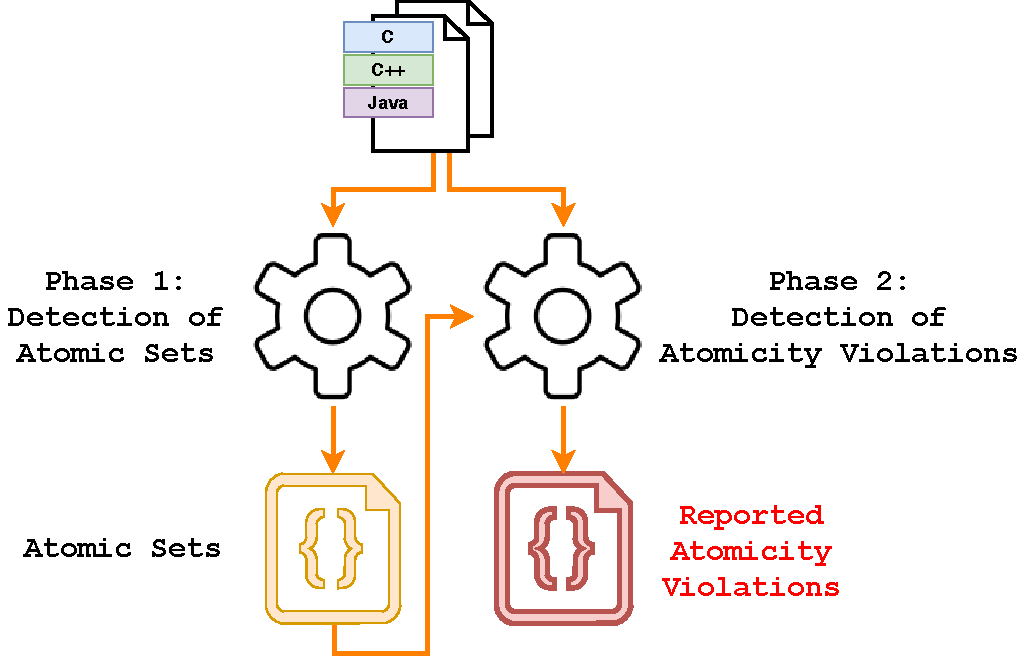
\includegraphics[width=.75 \linewidth]{analyser-proposal-sets.pdf}
    \caption{%
        An illustration of the \emph{phases} of the Atomer's analysis
        and the \emph{high-level analysis process} with an
        \emph{approximation} of working with \emph{sequences} by
        working with \emph{sets} (moreover, it can be visible that
        Atomer now accepts programs also written in \emph{C++} and
        \emph{Java} languages, which is described in
        Section~\ref{sec:implementLanguages})%
    }
    \label{fig:atomerPhasesSets}
\end{figure}

In particular, this proposed solution is more scalable because the order
of stored function calls is not relevant anymore while working with
sets. Therefore, less memory is required because the same sets of
function calls are not stored multiple times. The analysis is also faster
since there are stored fewer sets of function calls to work with. On the
other hand, the analysis is less accurate because the new approach
causes some loss of information. In practice, this loss of information
could eventually lead to \emph{false alarms}. However, the number of
such false alarms should not often be so significant. Moreover, later,
there are presented some techniques that try to rid of these false
alarms.

\subsection{%
    Approximation of the Abstract State and the Summary in Phase~1%
}

The \emph{detection of sequences of calls to be executed atomically} is now
based on analysing all paths through the CFG of a~function and generating
all pairs $ {(A, B)} \in 2^\Sigma \times 2^\Sigma $ (where~$ \Sigma $ is
a~set of all function names in a~given program) of \textbf{sets} of
function calls for each path. Here,~$ A, B $ are not \emph{reduced
sequences} (the notion of a~reduced sequence is not needed anymore), but sets,
and their semantics is preserved. So, the \emph{abstract state} $ s \in
\boldsymbol{Q} $ is redefined as $ 2^{2^{2^\Sigma \times 2^\Sigma}} $.

Further, in all the defined algorithms and definitions, it is
sufficient to work with:
\begin{itemize}
    \item 
        \emph{sets} of functions~$ 2^\Sigma $, instead of \emph{sequences}
        of functions~$ \Sigma^* $;
        
    \item
        \emph{empty sets}~$ \emptyset $, instead of \emph{empty
        sequences}~$ \varepsilon $;
        
    \item
        and \emph{union} of sets~$ \cup $, instead of a~\emph{concatenation}
        of sequences~$ \cdot $.
\end{itemize}
The above implies that the \emph{initial abstract state} of a~function is
changed to $ s_{init} = {\{\{{(\emptyset, \emptyset)}\}\}} $.
During the analysis of a~function~\texttt{g} with an abstract
state~$ s_\mathtt{g} $, when a~leaf function~\texttt{f} is called, the
abstract state's transformation is changed as follows:
$ s_\mathtt{g} = \{p^\prime \in 2^{2^\Sigma \times
2^\Sigma}\ |\ \exists\,p \in s_\mathtt{g} : p^\prime =
\textcolor{blue}{\{}{(A^\prime, B^\prime)} \in 2^\Sigma \times 2^\Sigma\ |\
\exists\,{(A, B)} \in p : \textcolor{violet}{(}\neg actual(p, (A, B)) \wedge
{(A^\prime, B^\prime)} = {(A, B)}\textcolor{violet}{)} \vee
\textcolor{red}{[}{actual(p, {(A, B)})} \wedge \textcolor{green}{[}(lock
\wedge {(A^\prime, B^\prime)} = {(A, B \cup \{\mathtt{f}\})}) \vee
(\neg lock \wedge {(A^\prime, B^\prime)} = {(A \cup \{\mathtt{f}\},
B)})\textcolor{green}{]}\textcolor{red}{]}\textcolor{blue}{\}}\} $. Further,
when an unlock is called, a~new ${ (A, B) }$ pair is created as follows:
$ s_\mathtt{g} = \{p^\prime \in 2^{2^\Sigma \times 2^\Sigma}\ |\ \exists\,p
\in s_\mathtt{g} : p^\prime = \textcolor{blue}{\{}{(A^\prime, B^\prime)}
\in 2^\Sigma \times 2^\Sigma\ |\ \textcolor{violet}{(}{(A^\prime, B^\prime)}
= {(\emptyset, \emptyset)} \wedge setActual(p, {(A^\prime,
B^\prime)})\textcolor{violet}{)} \vee {(A^\prime, B^\prime)} \in
p\textcolor{blue}{\}}\} $. Other definitions (e.g. calling an already
analysed \emph{nested} function) will be modified analogically.

Another approximation was made in \emph{summaries}. The first component
of the summary has to be changed to a~set of sets of function calls
because it is constructed from the~$ B $ items from abstract states,
which are now sets. The second component of the summary can be changed
to a~set of function calls, because even before, it was a~reduced
sequence of all the ${ (A, B) }$ pairs. Therefore, the order of function calls
was significantly approximated even so. Moreover, it is used to analyse
functions higher in the \emph{call hierarchy} where it is appended to~$ A $
or~$ B $, which are now sets. Thus, it would make no sense to store it in 
summaries as a~sequence. Formally, the summary~$ \chi_\mathtt{f} \in
2^{2^\Sigma} \times 2^\Sigma $ of a~function~\texttt{f} is redefined as
$ \chi_\mathtt{f} = (\boldsymbol{B}, AB) $, where:
\begin{itemize}
    \item 
        $ \boldsymbol{B} = \{B^\prime \in 2^\Sigma\ |\ \exists\,p \in
        s_\mathtt{f} : \exists\,{(A, B)} \in p : B \neq \emptyset \wedge
        B^\prime = B\} $, where~$ s_\mathtt{f} $ is the abstract state at
        the end of an interpretation of~\texttt{f}.
        
    \item
        $ AB = \bigcup\limits_{ab \in AB^\prime} ab $,
        where $ AB^\prime = \{ab \in 2^\Sigma\ |\ \exists\,p \in
        s_\mathtt{f} : \exists\,(A, B) \in p: ab = {A \cup B}\} $.
\end{itemize}

\begin{example}
    For demonstrating the approximation of the analysis with sets,
    assume functions~\texttt{f} and~\texttt{g} from
    Listing~\ref{list:atomerPhase1Sets}. Further assume,
    that~\texttt{a}, \texttt{b}, \texttt{x}, \texttt{y} are leaf
    nodes of the \emph{call graph}. Before the approximation,
    when the analysis was working with sequences of function calls,
    \textbf{Phase~1} of the analysis produced the following
    abstract states and summaries while analysing the functions:
    \begin{itemize}
        \item 
            $ s_\mathtt{f} = \{\{({(\mathtt{a}, \mathtt{b})}, {(\mathtt{x},
            \mathtt{y})}), ({(\mathtt{b}, \mathtt{a})}, {(\mathtt{y},
            \mathtt{x})}), {(\varepsilon, \varepsilon)}\}\} $,
            $ \chi_\mathtt{f} = (\{{(\mathtt{x}, \mathtt{y})},
            {(\mathtt{y}, \mathtt{x})}\}, (\mathtt{a}, \mathtt{b},
            \mathtt{x}, \mathtt{y})) $;
            
        \item
            $ s_\mathtt{g} = \{\{({(\mathtt{b}, \mathtt{a})},
            {(\mathtt{y}, \mathtt{x})}), {(\varepsilon,
            \varepsilon)}\}\} $, $ \chi_\mathtt{g} = (\{{(\mathtt{y},
            \mathtt{x})}\}, {(\mathtt{b}, \mathtt{a}, \mathtt{y},
            \mathtt{x})}) $.
    \end{itemize}
    Whereas, after the approximation, the produced abstract states
    and summaries are as follows (i.e. there is only one \uv{atomic set},
    and the summaries and abstract states are the same for both functions
    because there are the same locked/unlocked function calls, only the
    order of calls is different):
    \begin{itemize}
        \item 
            $ s_\mathtt{f} = \{\{({\{\mathtt{a}, \mathtt{b}\}},
            {\{\mathtt{x}, \mathtt{y}\}}), {(\emptyset, \emptyset)}\}\} $,
            $ \chi_\mathtt{f} = ({\{\{\mathtt{x}, \mathtt{y}\}\}},
            {\{\mathtt{a}, \mathtt{b}, \mathtt{x}, \mathtt{y}\}}) $;
            
        \item
            $ s_\mathtt{g} = \{\{({\{\mathtt{a}, \mathtt{b}\}},
            {\{\mathtt{x}, \mathtt{y}\}}), {(\emptyset, \emptyset)}\}\} $,
            $ \chi_\mathtt{g} = ({\{\{\mathtt{x}, \mathtt{y}\}\}},
            {\{\mathtt{a}, \mathtt{b}, \mathtt{x}, \mathtt{y}\}}) $.
    \end{itemize}
\end{example}

\begin{lstlisting}[
    style=c, label={list:atomerPhase1Sets}, float=hbt,
    caption={%
        A~code snippet used to illustrate the Atomer's
        \textbf{Phase~1} \emph{approximation} of the analysis with
        \emph{sets of function calls}%
    }
]
void f()
{
    a(); b();

    <@\textcolor{red}{pthread\_mutex\_lock}@>(&lock); // (x, y) -> {x, y}
    x(); y();
    <@\textcolor{red}{pthread\_mutex\_unlock}@>(&lock);
    
    b(); a();

    <@\textcolor{red}{pthread\_mutex\_lock}@>(&lock); // (y, x) -> {x, y}
    y(); x();
    <@\textcolor{red}{pthread\_mutex\_unlock}@>(&lock);
}
void g()
{
    b(); a();

    <@\textcolor{red}{pthread\_mutex\_lock}@>(&lock); // (y, x) -> {x, y}
    y(); x();
    <@\textcolor{red}{pthread\_mutex\_unlock}@>(&lock);
}
\end{lstlisting}

\subsection{Approximation with Sets in Phase~2}

\emph{Detecting violations of atomicity} works almost the same way as
before the approximation. There is only one difference. Before the
approximation, it was detected violations of atomic sequences obtained
from \textbf{Phase~1}. Now, \textbf{atomic sets} are obtained; hence,
detection of violations of atomic sets is performed. Again, the analysis
looks for \emph{pairs of functions that should be called atomically} while
this is not the case on some path through the CFG. This algorithm is
identical to the algorithm before the approximation.

Nevertheless, it is needed to propose a~new algorithm that derives the
pairs of function calls (from the atomic sets) to be checked for atomicity
(i.e. the set~$ \Omega \in 2^{\Sigma \times \Sigma} $). In order to obtain the
pairs, it is taken a~union of sets that contain all 2-element \emph{variations}
of single atomic sets (i.e. all the possible pairs). Formally, let~$ Q $ be
an analysed program, and let $ X_Q \in 2^{2^{2^\Sigma} \times 2^\Sigma} $ be
a~set of all \emph{summaries} of the program~$ Q $. Then, all the atomic pairs
(the first item of a~pair may be empty if an atomic set consists of a~single
function) are obtained as follows: $ \Omega = \{{(\mathtt{x}, \mathtt{y})}
\in \Sigma \times \Sigma\ |\ \exists\,{(\boldsymbol{B}, AB)} \in X_Q :
\exists\,B \in \boldsymbol{B} : (|B| = 1 \wedge {(\mathtt{x}, \mathtt{y})} \in
\{\varepsilon\} \times B) \vee (|B| > 1 \wedge {(\mathtt{x}, \mathtt{y})} \in
B \times B \wedge \mathtt{x} \neq \mathtt{y})\} $.

\begin{example}
    For example, assume that in \textbf{Phase~1}, there was analysed
    a~function~\texttt{f}, which produced the summary $ \chi_f =
    {(\boldsymbol{B}, AB)} $. Assume that before the approximation,
    a~set of sequences of functions that should be called atomically was
    as follows: $ \boldsymbol{B} = \{{(\mathtt{a}, \mathtt{b},
    \mathtt{c})}\} $. Then, the analysis looked for the following
    pairs of functions that are not called atomically: $ \Omega =
    \{{(\mathtt{a, b})}, {(\mathtt{b, c})}\} $. Since the result of the
    first component of the summary was changed to the following set of
    sets: $ \boldsymbol{B} = \{{\{\mathtt{a}, \mathtt{b}, \mathtt{c}\}}\} $,
    the analysis now looks for the following pairs  of functions that are not
    called atomically (all 2-element variations): $ \Omega = \{{(\mathtt{a},
    \mathtt{b})}, {(\mathtt{a}, \mathtt{c})}, {(\mathtt{b}, \mathtt{a})},
    {(\mathtt{b}, \mathtt{c})}, {(\mathtt{c}, \mathtt{a})}, {(\mathtt{c},
    \mathtt{b})}\} $.
\end{example}


\section{Advanced Manipulation with Locks}
\label{sec:proposalAdvancedLocks}

In the first version of Atomer, \emph{different locks} are not distinguished
at all. Only calls of locks/unlocks are identified, and parameters of these
calls (\emph{lock objects}) are not considered. In order to consider lock
objects, it was proposed distinguishing between them using Facebook Infer's
built-in mechanism called \emph{access paths}, explained in
Section~\ref{sec:accessPath}. The analyser does not perform a~general
\emph{alias analysis}, i.e., it is not performed a~precise analysis for
saying when arbitrary pairs of accesses to lock objects may alias. During
the analysis (both phases), each \emph{atomic section} is identified by an
access path of a~lock that guards the section, see
Sections~\ref{sec:proposalMultiLocksPhase1}, \ref{sec:proposalMultiLocksPhase2}.
Because \emph{syntactically identical access paths} are used as the intuition
for distinguishing atomic sections, some \emph{atomicity violations} could be
missed (or some \emph{false alarms} could be reported) due to distinct access
paths that refer to the same memory. However, it vastly simplifies the
analysis, and the stress is put on finding likely violations.

\subsection{Access Paths}
\label{sec:accessPath}

The \emph{syntactic access paths}~\cite{accessPath} represent \emph{heap
locations} via the paths used to access them, i.e., a~base variable followed
by a~sequence of fields. More formally, let $ Var $ be a~set of all variables
that can occur in a~given program. Let $ Field $ be a~set of all possible
field names that can be used in a~given program (e.g. structure fields). Then,
an access path~$ \pi $ from the set~$ \Pi $ of all access paths is defined
as follows:
$$
    \pi \in \Pi \Coloneqq Var \times Field^*
$$

Access paths are already implemented in Facebook Infer. For instance, the
principle of using access paths is used in an existing analyser in Facebook
Infer\,---\,RacerD~\cite{racerD}\,---\,for data race detection. In general,
no sufficiently precise \emph{alias analysis} works \emph{compositionally}
and at \emph{scale}. That is the motivation for using access paths in
Facebook Infer.

Given a~pair of accesses to lock objects, to determine whether these locks
are equal, it is needed to answer the following question: \uv{Can the
accesses touch the same address?}. Remarkably, according to the authors
of~\cite{racerD}, access paths alone \emph{almost} convey enough semantic
information to answer the above question on their own. If two access paths
are syntactically equal, it is almost (but not quite) true that they must
refer to the same address. Syntactically identical paths can refer to
different addresses if
\begin{enumerate*}[label={(\roman*)}]
    \item
        they refer to different instances of the same object or

    \item
        a~prefix of the path is reassigned along one execution trace,
        but not the other.
\end{enumerate*}
These conditions cannot hold if an access path is \emph{stable}, i.e., if
none of its proper prefixes appears in assignments during a~given
execution trace, then it touches the same memory as all other stable
accesses to the syntactic path. So, access paths' syntactic equality is
a~reasonably efficient way to say (in an \emph{under-approximate fashion})
that heap access touches the same address. Also, by using access paths,
RacerD detected many errors in real-world programs, proving that the
use of access paths can reveal real errors. This is why it was decided to
use this principle to represent locks in Atomer.

\subsection{Distinguishing Multiple Locks in Phase~1}
\label{sec:proposalMultiLocksPhase1}

The \emph{detection of sets of calls to be executed atomically} is based on
generating all pairs $ {(A, B)} \in 2^\Sigma \times 2^\Sigma $. Now, it is
needed to store \emph{access paths} of locks that guard calls
executed atomically, i.e., the~$ B $ sets. Therefore, these pairs are
extended to the triples $ {(A, B, \pi)} \in 2^\Sigma \times 2^\Sigma \times
\Pi $, where the third component is an access path that identifies
a~\emph{lock object} which locks an atomic section that contains the calls
from~$ B $. Note, that~$ \pi $ could also be~$ \varepsilon $ (i.e.
$ \varepsilon \in \Pi $), which is a~special case when there is no lock
associated to the~${ (A, B) }$ pair so far, i.e., $ B $ is empty as well,
and a~lock was not called yet. The \emph{abstract state} $ s \in
\boldsymbol{Q} $ is now defined as $ 2^{2^{2^\Sigma \times 2^\Sigma \times
\Pi}} $. When a~function is called, it is appended to the~$ A $
set of the triple where $ \pi = \varepsilon $, i.e., the triple without
an associated lock. Also, it is appended to all the triples that have
some lock which is currently locked. When a~lock is called, its identifier
is associated to the triple without any lock associated to it (which is
then labelled as the currently locked lock), and it is created a~new triple
without a~lock. Finally, when an unlock is called, it is created a~new
triple without a~lock, and all the currently locked locks are labelled
as unlocked.

Formally, the \emph{initial abstract state} of a~function is changed to
$ s_{init} = \{\{{(\emptyset, \emptyset, \varepsilon)}\}\} $. During the
analysis of a~function~\texttt{g} with an abstract state~$ s_\mathtt{g} $,
when a~leaf function~\texttt{f} is called, the abstract state's
transformation is changed as follows: $ s_\mathtt{g} = \{p^\prime \in
2^{2^\Sigma \times 2^\Sigma \times \Pi}\ |\ \exists\,p \in s_\mathtt{g}
: p^\prime = \textcolor{blue}{\{}{(A^\prime, B^\prime, \pi^\prime)} \in
2^\Sigma \times 2^\Sigma \times \Pi\ |\ \exists\,{(A, B, \pi)} \in p
: \textcolor{green}{(}\pi = \varepsilon \wedge {(A^\prime, B^\prime,
\pi^\prime)} = {(A \cup \{\mathtt{f}\}, B, \pi)}\textcolor{green}{)} \vee
\textcolor{red}{[}\pi \neq \varepsilon \wedge
\textcolor{green}{[}\textcolor{violet}{(}{(A, B, \pi)} \in locked(p)
\wedge {(A^\prime, B^\prime, \pi^\prime)} = {(A, B \cup \{\mathtt{f}\},
\pi)}\textcolor{violet}{)} \vee \textcolor{orange}{(}{(A, B, \pi)}
\notin locked(p) \wedge {(A^\prime, B^\prime, \pi^\prime)} = {(A, B,
\pi)}\textcolor{orange}{)}\textcolor{green}{]}\textcolor{red}{]}%
\textcolor{blue}{\}}\} $, where $ locked $ is a~function that returns
(for a~given program path) a~set of the ${ (A, B, \pi) }$ triples where
the lock identified by~$ \pi $ is currently locked. Further, when a~lock
identified by the access path~$ \pi_i $ is called, the abstract state
changes as follows: $ s_\mathtt{g} = \{
p^\prime \in 2^{2^\Sigma \times 2^\Sigma \times \Pi}\ |\ \exists\,p \in
s_\mathtt{g} : p^\prime = \textcolor{blue}{\{}{(A^\prime, B^\prime,
\pi^\prime)} \in 2^\Sigma \times 2^\Sigma \times \Pi\ |\ {(A^\prime,
B^\prime, \pi^\prime)} = {(\emptyset, \emptyset, \varepsilon)} \vee
\textcolor{violet}{(}{(A^\prime, B^\prime, \pi^\prime)} \in p \wedge
\pi^\prime \neq \varepsilon\textcolor{violet}{)} \vee
\textcolor{red}{[}{(A^\prime, B^\prime, \varepsilon)} \in p \wedge
\pi^\prime = \pi_i \wedge setLocked\textcolor{green}{(}p,
locked(p) \cup \{{(A^\prime, B^\prime, \pi^\prime)}\}\textcolor{green}{)}%
\textcolor{red}{]}\textcolor{blue}{\}}\} $, where $ setLocked $ is
a~function that labels triples (for a~given program path) as those currently
locked by their lock. Furthermore, when an unlock identified by the access
path~$ \pi_i $ is called, the abstract state changes as follows:
$ s_\mathtt{g} = \{p^\prime \in 2^{2^\Sigma \times 2^\Sigma \times \Pi}\
|\ \exists\,p \in s_\mathtt{g} : p^\prime = \textcolor{blue}{\{}{(A^\prime,
B^\prime, \pi^\prime)} \in 2^\Sigma \times 2^\Sigma \times \Pi\ |\
{(A^\prime, B^\prime, \pi^\prime)} = {(\emptyset, \emptyset, \varepsilon)}
\vee \textcolor{violet}{(}{(A^\prime, B^\prime, \pi^\prime)} \in p
\wedge \pi^\prime \neq \varepsilon \wedge \pi^\prime \neq
\pi_i\textcolor{violet}{)} \vee \textcolor{red}{[}{(A^\prime, B^\prime,
\pi^\prime)} \in p \wedge \pi^\prime = \pi_i \wedge
setLocked\textcolor{green}{(}p, locked(p) \setminus \{{(A^\prime,
B^\prime, \pi^\prime)}\}\textcolor{green}{)}\textcolor{red}{]}%
\textcolor{blue}{\}}\} $. Other definitions (e.g. calling and already
analysed \emph{nested} function) will be changed analogically.

The \emph{summary} $ \chi_\mathtt{f} \in 2^{2^\Sigma} \times 2^\Sigma $
of a~function~\texttt{f} is the same as earlier. Only access paths
from abstract states are ignored. I.e. $ \chi_\mathtt{f} = {(\boldsymbol{B},
AB)} $, where:
\begin{itemize}
    \item 
        $ \boldsymbol{B} = \{B^\prime \in 2^\Sigma\ |\ \exists\,p \in
        s_\mathtt{f} : \exists\,{(A, B, \pi)} \in p : B \neq \emptyset \wedge
        B^\prime = B\} $, where~$ s_\mathtt{f} $ is the abstract state at
        the end of an interpretation of~\texttt{f}.
        
    \item
        $ AB = \bigcup\limits_{ab \in AB^\prime} ab $,
        where $ AB^\prime = \{ab \in 2^\Sigma\ |\ \exists\,p \in
        s_\mathtt{f} : \exists\,(A, B, \pi) \in p: ab = {A \cup B}\} $.
\end{itemize}

\begin{example}
    Consider two base cases (\emph{nested atomic section} and
    \emph{alternating sequence of locks}) in function~\texttt{f}
    and~\texttt{g} from Listing~\ref{list:atomerPhase1MultiLocks}. There
    are two lock objects \texttt{lockA} and \texttt{lockB} that are used
    simultaneously. Further assume, that~\texttt{a}, \texttt{b},
    \texttt{c} are leaf nodes of the \emph{call graph}. After the
    extension of the distinguishment of multiple locks used,
    the produced abstract states and summaries are as follows:
    \begin{itemize}
        \item 
            $ s_\mathtt{f} = \{\{{(\{\mathtt{a}\}, \{\mathtt{b}\},
            \mathtt{lockB})}, {(\emptyset, \{\mathtt{a}, \mathtt{b},
            \mathtt{c}\}, \mathtt{lockA})}, {(\emptyset, \emptyset,
            \varepsilon)}\}\} $, \\
            $ \chi_\mathtt{f} = ({\{\{\mathtt{b}\}, \{\mathtt{a}, \mathtt{b},
            \mathtt{c}\}\}}, {\{\mathtt{a}, \mathtt{b}, \mathtt{c}\}}) $;

        \item 
            $ s_\mathtt{f} = \{\{{(\emptyset, \{\mathtt{a}, \mathtt{b}\},
            \mathtt{lockA})}, {(\{\mathtt{a}\}, \{\mathtt{b}, \mathtt{c}\},
            \mathtt{lockB})}, {(\emptyset, \emptyset, \varepsilon)}\}\} $, \\
            $ \chi_\mathtt{f} = ({\{\{\mathtt{a}, \mathtt{b}\}, \{\mathtt{b},
            \mathtt{c}\}\}}, {\{\mathtt{a}, \mathtt{b}, \mathtt{c}\}}) $.
    \end{itemize}
\end{example}

\begin{lstlisting}[
    style=c, label={list:atomerPhase1MultiLocks}, float=hbt,
    caption={%
        A~code snippet used to illustrate \emph{distinguishing
        multiple locks used} during derivation of \emph{sets
        of functions called atomically}%
    }
]
void f()
{
    <@\textcolor{red}{pthread\_mutex\_lock}@>(&<@\textcolor{magenta}{lockA}@>); // {a, b, c}
    a();
    <@\textcolor{red}{pthread\_mutex\_lock}@>(&<@\textcolor{cyan}{lockB}@>); // {b}
    b();
    <@\textcolor{red}{pthread\_mutex\_unlock}@>(&<@\textcolor{cyan}{lockB}@>);
    c();
    <@\textcolor{red}{pthread\_mutex\_unlock}@>(&<@\textcolor{magenta}{lockA}@>);
}
void g()
{
    <@\textcolor{red}{pthread\_mutex\_lock}@>(&<@\textcolor{magenta}{lockA}@>); // {a, b}
    a();
    <@\textcolor{red}{pthread\_mutex\_lock}@>(&<@\textcolor{cyan}{lockB}@>); // {b, c}
    b();
    <@\textcolor{red}{pthread\_mutex\_unlock}@>(&<@\textcolor{magenta}{lockA}@>);
    c();
    <@\textcolor{red}{pthread\_mutex\_unlock}@>(&<@\textcolor{cyan}{lockB}@>);
}
\end{lstlisting}

\subsection{Distinguishing Multiple Locks in Phase~2}
\label{sec:proposalMultiLocksPhase2}

The pairs~$ \Omega $ of functions that should be called atomically are
computed the same way as earlier during the \emph{detection of atomicity
violations} in \textbf{Phase~2}. The analysis again looks for \emph{pairs
of functions that should be called atomically} while this is not the case
on some path through the CFG. However, this time, there are stored (in addition
to a~pair of the most recent function calls) all the most recent pairs of
function calls locked under individual locks.

An \emph{abstract state} element is the following: $ {(\mathtt{x},
\mathtt{y}, \Delta, \Lambda)} \in \Sigma \times \Sigma \times 2^{\Sigma
\times \Sigma} \times 2^{\Sigma \times \Sigma \times \Pi} $, where
${ (\mathtt{x}, \mathtt{y}) }$ and~$ \Delta $ are as before. $ \Lambda $ is
a~set of \emph{locked pairs} of the most recent function calls with
their locks' \emph{access paths}. Thus, the abstract state $ s \in
\boldsymbol{Q} $ is defined as $ 2^{\Sigma \times \Sigma \times 2^{\Sigma
\times \Sigma} \times 2^{\Sigma \times \Sigma \times \Pi}} $. The analysis
works as follows. When a~function~\texttt{f} is called, it is created a~new
pair ${ (\mathtt{x}^\prime, \mathtt{y}^\prime) }$ of the most recent function
calls from the previous pair ${ (\mathtt{x}, \mathtt{y}) }$ (i.e.
$ {(\mathtt{x}^\prime, \mathtt{y}^\prime)} = {(\mathtt{y}, \mathtt{f})} $).
This pair is also stored to the locked pairs~$ \Lambda $ if there are any
locks currently locked. Further, it is checked whether the new pair (or
just the last call) violates atomicity, and at the same time, it is not
locked by any of the stored locks (i.e. $ ({(\mathtt{x}^\prime,
\mathtt{y}^\prime)} \in \Omega \wedge {(\mathtt{x}^\prime,
\mathtt{y}^\prime)} \notin \Lambda) \vee ({(\varepsilon, \mathtt{y}^\prime)}
\in \Omega \wedge {(\varepsilon, \mathtt{y}^\prime)} \notin \Lambda) $).
When it holds, it is added to the set~$ \Delta $ of pairs that violate
atomicity.

More formally, the \emph{initial abstract state} of a~function is defined
as $ s_{init} = {\{\{(\varepsilon, \varepsilon, \emptyset, \emptyset)\}\}} $.
To formalise the analysis of a~function, let~\texttt{f} be a~called leaf
function. Further, let~$ s_\mathtt{g} $ be the abstract state of
a~function~\texttt{g} being analysed before the function~\texttt{f} is
called. After the call of~\texttt{f}, the abstract state will be changed
as follows: $ s_\mathtt{g} = \{{(\mathtt{x}^\prime, \mathtt{y}^\prime,
\Delta^\prime, \Lambda^\prime)} \in \Sigma \times \Sigma \times
2^{\Sigma \times \Sigma} \times 2^{\Sigma \times \Sigma \times \Pi}\ |
\ \exists\,{(\mathtt{x}, \mathtt{y}, \Delta, \Lambda)} \in s_\mathtt{g} :
{(\mathtt{x}^\prime, \mathtt{y}^\prime)} = {(\mathtt{y}, \mathtt{f})}
\wedge \Lambda^\prime = \textcolor{blue}{\{}{(\mathtt{x}_\pi^\prime,
\mathtt{y}_\pi^\prime, \pi^\prime)} \in \Sigma \times \Sigma \times \Pi\ 
|\ \exists\,{(\mathtt{x}_\pi, \mathtt{y}_\pi, \pi)} \in \Lambda :
{(\mathtt{x}_\pi^\prime, \mathtt{y}_\pi^\prime, \pi^\prime)} =
{(\mathtt{y}_\pi, \mathtt{f}, \pi)}\textcolor{blue}{\}} \wedge
\Delta^\prime = \textcolor{red}{\{}{(\mathtt{x}^{\prime\prime},
\mathtt{y}^{\prime\prime})} \in \Sigma \times \Sigma\ |\
{(\mathtt{x}^{\prime\prime}, \mathtt{y}^{\prime\prime})} \in \Delta
\vee \textcolor{green}{[}\textcolor{violet}{(}{(\mathtt{x}^{\prime\prime},
\mathtt{y}^{\prime\prime})} = {(\mathtt{x}^\prime, \mathtt{y}^\prime)} \vee
{(\mathtt{x}^{\prime\prime}, \mathtt{y}^{\prime\prime})} = {(\varepsilon,
\mathtt{y}^\prime)}\textcolor{violet}{)} \wedge {(\mathtt{x}^{\prime\prime},
\mathtt{y}^{\prime\prime})} \in \Omega \wedge
\nexists\,{(\mathtt{x}^{\prime\prime}_\pi, \mathtt{y}^{\prime\prime}_\pi,
\pi^{\prime\prime})} \in \Lambda^\prime : {(\mathtt{x}^{\prime\prime}_\pi,
\mathtt{y}^{\prime\prime}_\pi)} = {(\mathtt{x}^{\prime\prime},
\mathtt{y}^{\prime\prime})}\textcolor{green}{]}\textcolor{red}{\}}\} $.
Further, when a~lock identified by the access path~$ \pi_i $ is called,
the abstract state is changed as follows: $ s_\mathtt{g} =
\{{(\mathtt{x}^\prime, \mathtt{y}^\prime, \Delta^\prime, \Lambda^\prime)}
\in \Sigma \times \Sigma \times 2^{\Sigma \times \Sigma} \times 2^{\Sigma
\times \Sigma \times \Pi}\ |\ \exists\,{(\mathtt{x}, \mathtt{y}, \Delta,
\Lambda)} \in s_\mathtt{g} : {(\mathtt{x}^\prime, \mathtt{y}^\prime,
\Delta^\prime, \Lambda^\prime)} = {(\mathtt{x}, \mathtt{y}, \Delta,
\Lambda \cup {\{(\varepsilon, \varepsilon, \pi_i)\}})}\} $. Furthermore,
when an unlock identified by the access path~$ \pi_i $ is called, the
abstract state is changed as follows: $ s_\mathtt{g} =
\{{(\mathtt{x}^\prime, \mathtt{y}^\prime, \Delta^\prime, \Lambda^\prime)}
\in \Sigma \times \Sigma \times 2^{\Sigma \times \Sigma} \times 2^{\Sigma
\times \Sigma \times \Pi}\ |\ \exists\,{(\mathtt{x}, \mathtt{y}, \Delta,
\Lambda)} \in s_\mathtt{g} : {(\mathtt{x}^\prime, \mathtt{y}^\prime,
\Delta^\prime, \Lambda^\prime)} = {(\mathtt{x}, \mathtt{y}, \Delta,
\Lambda \setminus \Sigma \times \Sigma \times \{\pi_i\})}\} $.

\begin{example}
    Consider the function~\texttt{f} from
    Listing~\ref{list:atomerPhase2MultiLocks}. There are two lock objects
    \texttt{lockA} and \texttt{lockB} that are used simultaneously.
    Further assume, that~\texttt{a}, \texttt{b} are leaf nodes of the
    \emph{call graph}. Then assume, that the result of the first
    phase of the analysis is that a~pair of functions~\texttt{a},
    \texttt{b} that should be called atomically, i.e., $ \Omega =
    {\{(\mathtt{a}, \mathtt{b})\}} $. Before the extension of
    the distinguishment of multiple locks used, the analysis
    would report an atomicity violation of these functions (line~6).
    That is because the locks are not distinguished, and the
    unlock of \texttt{lockA} (line~5) would unlock everything.
    On the other hand, after the extension, there are not reported
    any atomicity violations because the pair of functions is
    locked using the second lock\,---\,\texttt{lockB}. The abstract
    state~$ s_\mathtt{f} $ of the function~\texttt{f} before
    line~7 looks like follows: $ s_\mathtt{f} = \{{(\mathtt{a},
    \mathtt{b}, \emptyset, \{(\mathtt{a}, \mathtt{b},
    \mathtt{lockB})\})}\} $.
\end{example}

\begin{lstlisting}[
    style=c, label={list:atomerPhase2MultiLocks}, float=hbt,
    caption={%
        A~code snippet used to illustrate \emph{distinguishing
        multiple locks used} during \emph{detection of atomicity
        violations}%
    }
]
void f()
{
    <@\textcolor{red}{pthread\_mutex\_lock}@>(&<@\textcolor{magenta}{lockA}@>); // {}
    <@\textcolor{red}{pthread\_mutex\_lock}@>(&<@\textcolor{cyan}{lockB}@>); // {a, b}
    <@\textcolor{red}{pthread\_mutex\_unlock}@>(&<@\textcolor{magenta}{lockA}@>);
    a(); b();
    <@\textcolor{red}{pthread\_mutex\_unlock}@>(&<@\textcolor{cyan}{lockB}@>);
}
\end{lstlisting}


\section{Analysis's Parametrisation}
\label{sec:proposalParametr}


\section{Local/Global Atomicity Violations}
\label{sec:proposalLocalGlobalViols}



%===============================================================================


\chapter{Implementation of a~New Version of Atomer}
\label{chap:implement}

\todo{Některé věci částečně převzít z~projektové praxe a~z~Excelu. Zmínit, že byl aktualizován Infer a~že byl udělán nějaký refaktoring.}


\section{\texorpdfstring{Phase~1\,---\,Detection of Atomic Sets}{Phase~1 - Detection of Atomic Sets}}
\label{sec:implementPhase1}


\section{\texorpdfstring{Phase~2\,---\,Detection of Atomicity Violations}{Phase~2 - Detection of Atomicity Violations}}
\label{sec:implementPhase2}


\section{Support for C++ and Java Languages}
\label{sec:implementLanguages}


\section{Additional Locking Mechanisms}
\label{sec:implementLocks}



%===============================================================================



\chapter{Experimental Evaluation of the New Version of Atomer}
\label{chap:exp}

\todo{Některé věci převzít z~Excelu a~z~projektové praxe.}


\section{Testing on Hand-Crafted Examples}
\label{sec:expHand}


\section{Scalability Benchmark}
\label{sec:expScal}


\section{Evaluation on Validation Programs Derived from Gluon}
\label{sec:expGluon}


\section{Experiments with Real-Life Programs}
\label{sec:expReal}


\section{Summary of the Evaluation and Future Work}
\label{sec:expSummary}



%===============================================================================



\chapter{Conclusion}
\label{chap:conc}

This thesis started by describing the principles of \emph{static analysis}
and \emph{abstract interpretation}. Further, \emph{Facebook Infer} was
described\,---\,a~concrete static analysis framework that uses abstract
interpretation\,---\,its features, architecture, and existing analysers
implemented in this tool. Next, there were described \emph{contracts for
concurrency}. The major part of the thesis then aimed at the description of
static analyser \emph{Atomer}\footnote{The implementation of \textbf{Atomer}
is available on GitHub as an \emph{open-source} repository (in a~branch
\texttt{atomicity-sets}):
\url{https://github.com/harmim/infer}.}\,---\,proposed and implemented
within the author's bachelor's thesis~\cite{harmimBP}\,---\,implemented as
a~Facebook Infer's module, and that detects \emph{atomicity violations}.
It was described its limitations, and thereafter, it was described the
proposal and implementation of its extensions and improvements. Lastly,
the experimental evaluation of the new features and improvements was
depicted, and there were also described other performed experiments
and possible future work.

Atomer works on the level of \emph{sequences of function calls}. It is
based on the assumption that sequences of function calls executed
\emph{atomically once} should probably be executed \emph{always atomically},
and it naturally works with sequences. In the thesis, to improve
\emph{scalability}, the use of sequences was \emph{approximated} by
\emph{sets}. Further, two new features were implemented: support for
\emph{C++} and \emph{Java} languages; and distinguishing \emph{multiple
locks used}.

The introduced enhancements were successfully tested on \emph{hand-crafted}
programs. It turned out that such innovations improved the \emph{accuracy}
and \emph{scalability}. Moreover, Atomer was experimentally evaluated on
additional software. Notably, it was evaluated on \emph{real-life Java
programs}\,---\,\emph{Apache Cassandra} and \emph{Tomcat}. Already fixed
and reported \emph{real bugs} were successfully rediscovered. Nevertheless,
so far, quite some \emph{false alarms} are reported.

Several other improvements were proposed to reduce the number of false
alarms, namely, \emph{parametrisation} of the analysis, support for
\emph{interprocedural locks}, or combinations with a~\emph{dynamic analysis}.
Their implementation and evaluation is currently the work in progress.

Atomer's \emph{accuracy} can be further increased. Some of its limitations
and possible solutions are discussed in this thesis, e.g., considering
\emph{formal parameters} and distinguishing the \emph{context} of
called functions, \emph{ranking} of atomic functions, or focusing on
\emph{library containers concurrency restrictions} related to method
calls. Further, it is needed to perform more experiments on \emph{real-life}
programs to find and report \emph{new bugs}.



%===============================================================================



    % Bibliography
    % --------------------------------------------------------------------------
    \makeatletter
    \def\@openbib@code{\addcontentsline{toc}{chapter}{Bibliography}}
    \makeatother
    \bibliographystyle{enplain}

    \begin{flushleft}
        \bibliography{xharmi00}
    \end{flushleft}


    \iftwoside\cleardoublepage\else\clearpage\fi


    % Appendices
    % --------------------------------------------------------------------------
    \appendix
    %===============================================================================
% (c) Dominik Harmim

\todo{Možná přidat přílohu s~výstupem
analyzátoru v~různých formátech (kvůli propojení s~dynamickou analýzou.)}



%===============================================================================
\chapter{Experimental Validation}
\label{app:expValid}

\todo{Možná přidat ještě nějaké validační příklady. Jinak strukturu asi
převzít z~bakalářky a~kód z~mých repositářů.}


\section{Validation of the Approximation with Sets of Calls}
\label{sec:validSets}


\section{Validation of the Support for C++ and Java Locks}
\label{sec:validLanguages}



%===============================================================================
\chapter{Contents of the Attached Memory Media}
\label{app:memMedia}

\todo{Strukturu převzít z~bakalářky.}



%===============================================================================
\chapter{Installation and User Manual}
\label{app:man}

\todo{Převzít z~bakalářky a~aktualizovat, hlavně přidat použití parametrů
analyzátoru.}


\section*{Installation Manual}


\section*{User Manual}



%===============================================================================

\end{document}
